% Universidade Aberta
% Template TeX para relatório de trabalhos
% 2025
%
%
% Dados para a capa
\newcommand{\Titulo}{Planeamento e Desenvolvimento de Sistemas de Informação}
\newcommand{\SubTitulo}{Trabalho Grupo - Projeto Final}
\newcommand{\Ano}{2025}
\newcommand{\Autor}{
    Pedro Morais - 2401849 \\
    Hugo Gonçalves - 2100562 \\
    Pedro Moro - 2001642 \\
    Luis Peixoto - 2402741 \\
}
%
%
\documentclass[12pt,a4paper,final]{article}
\usepackage{csquotes}
\usepackage{float}
\usepackage[portuguese]{babel}
\usepackage{polyglossia}
\usepackage{longtable}
\setdefaultlanguage{portuguese}
\usepackage{graphicx}
\graphicspath{ {./images/} }
\usepackage[a4paper,top=3cm,bottom=3cm,left=3.5cm,right=2cm]{geometry}
\usepackage{booktabs}
\setmainfont{Times New Roman}
\defaultfontfeatures{Ligatures=TeX}
\usepackage[pdfauthor=\Autor,
    pdftitle=\Titulo,
    colorlinks=true,
    linkcolor=black,
    citecolor=black,
    bookmarksopen=true]{hyperref}
\hypersetup{colorlinks, citecolor=black, urlcolor=black}
\usepackage{bookmark}
\usepackage[style=apa, backend=biber, sortcites, url=true, language=portuguese]{biblatex}
\usepackage{fontspec}
\DeclareLanguageMapping{portuguese}{portuguese-apa}
\addbibresource{ref.bib}
\renewcommand{\baselinestretch}{1.5}
\begin{document}
    \title{\Titulo}
    \author{\Autor}
    \date{\Ano}
    \pagenumbering{gobble}
    \begin{titlepage}
        \begin{center}
            \vspace*{4cm}

            \textbf{\large UNIVERSIDADE ABERTA}

            \textbf{\large UNIVERSIDADE DE TRÁS-OS-MONTES E ALTO DOURO}

            \vspace{1cm}

            \begin{minipage}{0.4\textwidth}
                \centering
                
\includegraphics[width=0.8\textwidth]{uab}
            \end{minipage}
            \begin{minipage}{0.4\textwidth}
                \centering
                
\includegraphics[width=0.8\textwidth]{utad}
            \end{minipage}

            \vspace{1.5cm}

            \textbf{\large \Titulo}

            \textbf{\large \SubTitulo}

            \vspace{1.5cm}

            \textbf{\large \Autor}

            \vspace{2cm}

            \textbf{\large Mestrado em Engenharia Informática e Tecnologia Web}
            \vfill
            \textbf{\Ano}
        \end{center}
    \end{titlepage}
    \renewcommand{\contentsname}{Índice}
    \cleardoublepage
    \pagenumbering{roman}
    \tableofcontents
    \newpage
    \listoffigures
    \newpage
    \listoftables
    \newpage
    \cleardoublepage
    \pagenumbering{arabic}

    \section*{Introdução}
    \addcontentsline{toc}{section}{Introdução}

    O presente relatório foi elaborado no âmbito da unidade curricular de Planeamento e Desenvolvimento de Sistemas de Informação, tendo como objeto de estudo a Direção Municipal de Higiene Urbana (DMHU) da Câmara Municipal de Lisboa. O objetivo fundamental consistiu em caracterizar detalhadamente a arquitetura empresarial “AS-IS”, identificar fragilidades e lacunas nos sistemas de informação atuais e, com base nessa análise, propor uma arquitetura “TO-BE” robusta, escalável e alinhada com as melhores práticas de modernização administrativa e digital.

    Foram seguidas metodologias reconhecidas internacionalmente, nomeadamente ArchiMate 3, BPMN 2.0 e UML 2.0, apoiando a modelação e documentação dos processos, entidades, aplicações e infraestruturas. Cada questão do enunciado foi cuidadosamente tratada, recorrendo a modelos visuais, matrizes, análises críticas e fundamentação teórica, sempre tendo em consideração o feedback contínuo do professor orientador.

    Este relatório visa, assim, fornecer uma base sólida para a transformação digital da DMHU, identificando não apenas o estado atual, mas também um caminho exequível e fundamentado para a evolução da arquitetura, a eliminação de silos, a promoção da interoperabilidade e o alinhamento com os desafios de uma “Smart City”.


    \section*{Questão 1 – Contexto da DMHU}
    \addcontentsline{toc}{section}{Q1 – Contexto da DMHU}

    O diagrama de contexto apresentado ilustra os principais atores internos e externos que interagem com a Direção Municipal de Higiene Urbana (DMHU). Conforme o feedback recebido, foi feita a correção de incluir a DMHU como caixa central e representar os departamentos internos e a sua interação com outras áreas da Câmara Municipal de Lisboa.

    \begin{figure}[H]
        \centering
        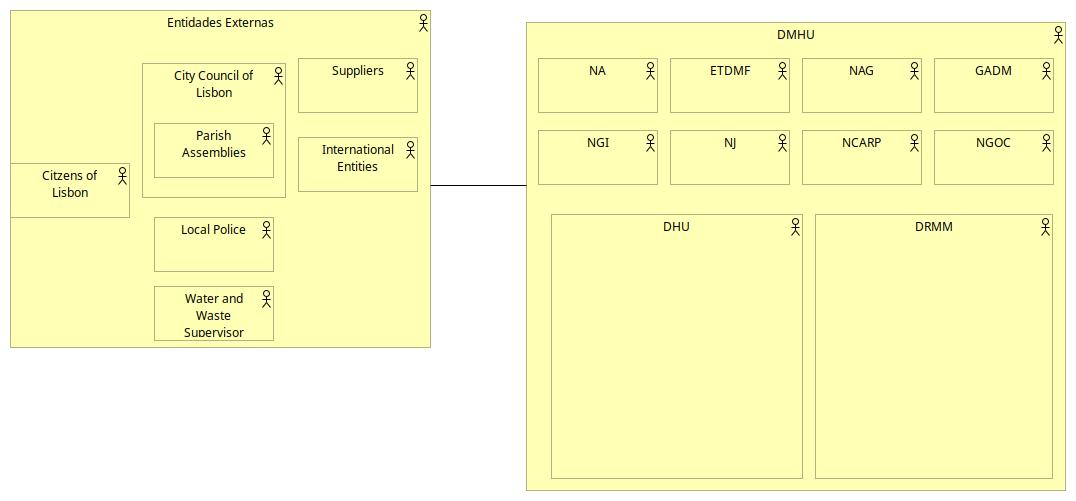
\includegraphics[width=0.9\textwidth]{Q1a - DMHU Context.jpg}
        \caption{Contexto organizacional da DMHU com atores internos e externos}
        \label{fig:q1-contexto}
    \end{figure}

    \section*{Questão 2 – Produtos e Serviços}
    \addcontentsline{toc}{section}{Q2 – Produtos e Serviços}

    A DMHU presta um vasto conjunto de serviços, desde a recolha de resíduos, limpeza urbana, sensibilização ambiental, entre outros. O diagrama foi revisto de acordo com o feedback, e inclui agora atores como a UHU, DLU e DRMM representados como áreas internas à DMHU.

    \begin{figure}[H]
        \centering
        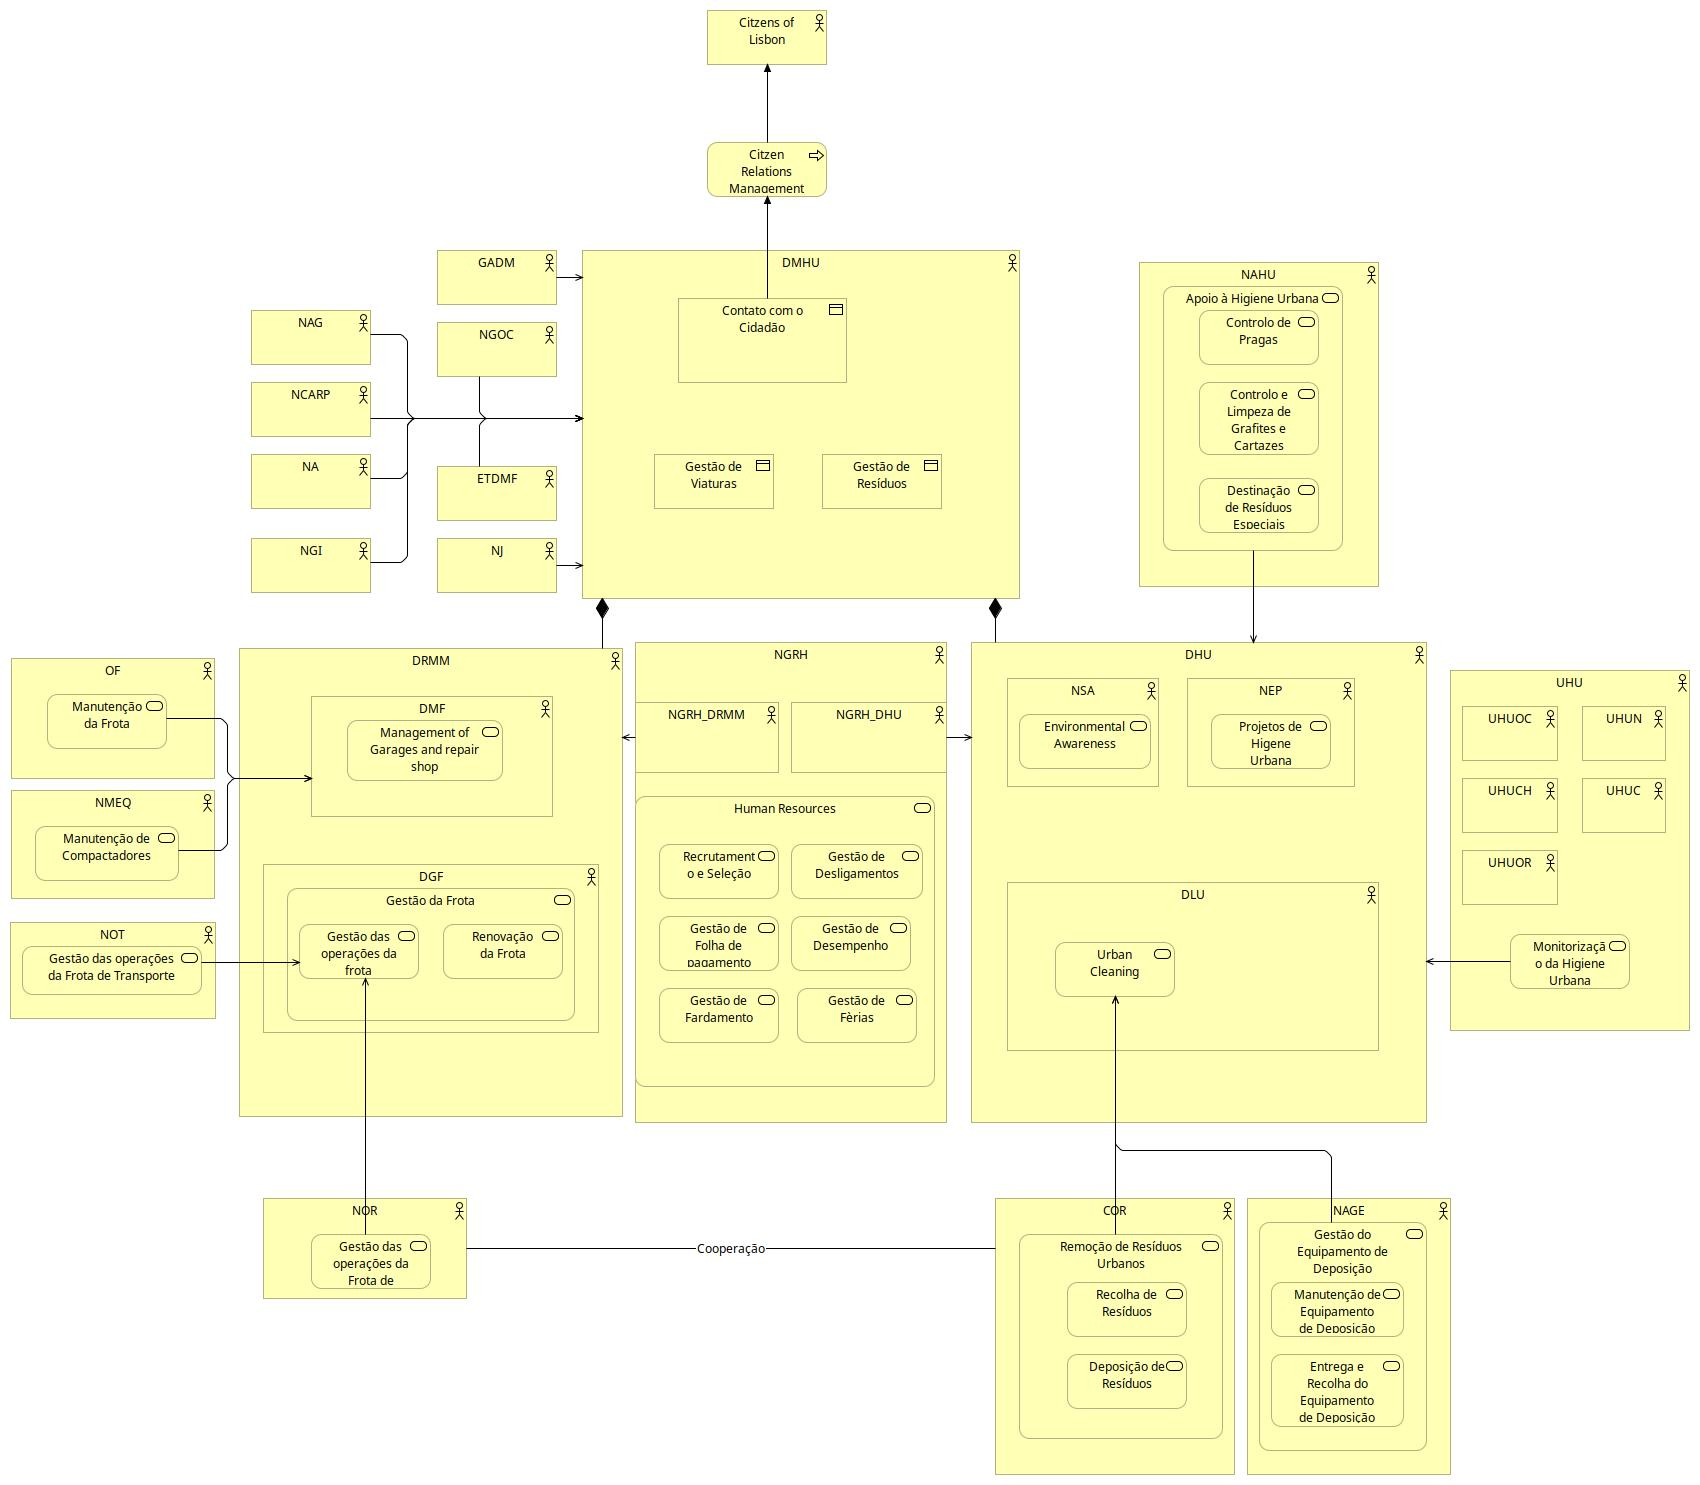
\includegraphics[width=0.9\textwidth]{Q2 - Business Products and services.jpg}
        \caption{Produtos e serviços prestados pela DMHU}
        \label{fig:q2-servicos}
    \end{figure}

    \section*{Questão 3 – Estrutura Organizacional}
    \addcontentsline{toc}{section}{Q3 – Estrutura Organizacional}

    A estrutura organizacional apresentada contempla os dois departamentos da DMHU: Higiene Urbana e Reparação e Manutenção, com os respetivos centros de apoio, divisões e estruturas transversais. A unidade UHU foi integrada no diagrama principal, conforme sugestão do professor.

    \begin{figure}[H]
        \centering
        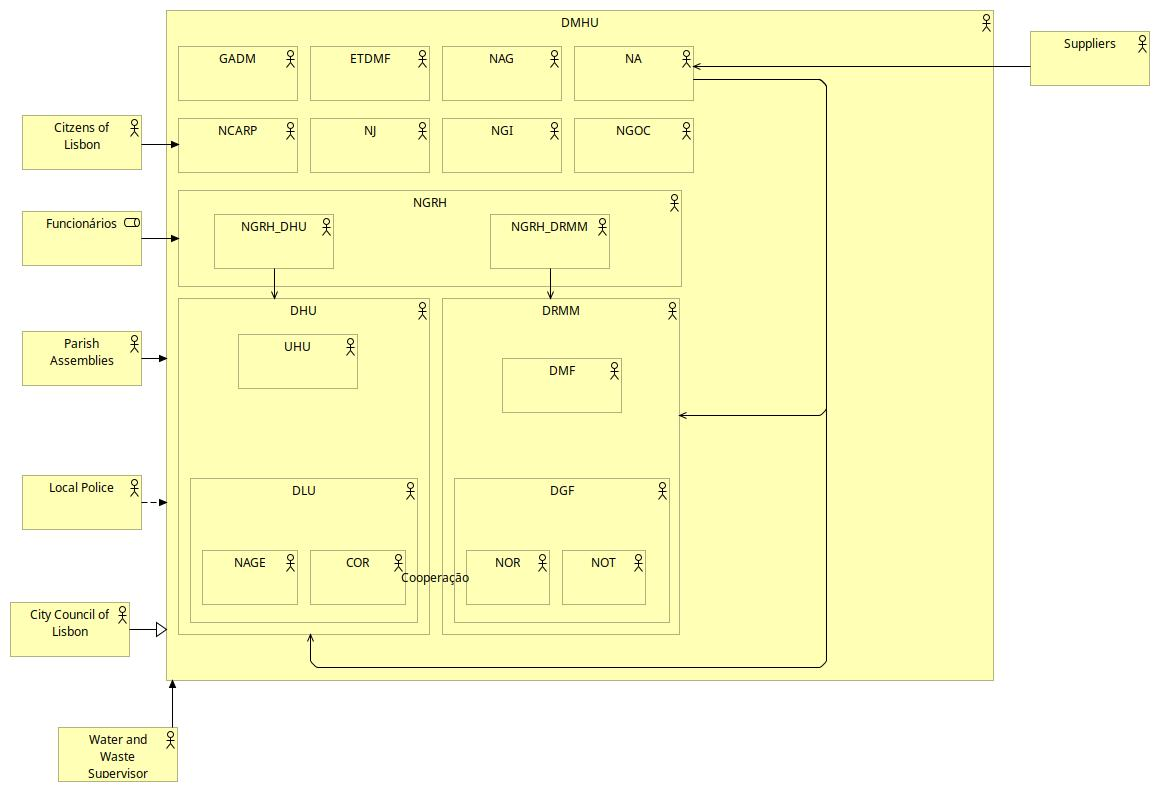
\includegraphics[width=0.9\textwidth]{Q3 - Business Cooperation.jpg}
        \caption{Estrutura organizacional da DMHU}
        \label{fig:q3-organizacao}
    \end{figure}

    \section*{Questão 4 – Relação entre Serviços e Processos de Negócio}
    \addcontentsline{toc}{section}{Q4 – Relação entre Serviços e Processos de Negócio}

    O conjunto de diagramas seguintes representa a ligação entre os principais serviços de negócio da DMHU e os respectivos processos, destacando-se as áreas fulcrais: Armazém, Frota, Relação com o Cidadão, Resíduos e Recursos Humanos. Em resposta ao feedback do professor, foram incluídas mais ligações entre processos, reflectindo a interdependência operacional e a exposição dos serviços.

    \begin{figure}[H]
        \centering
        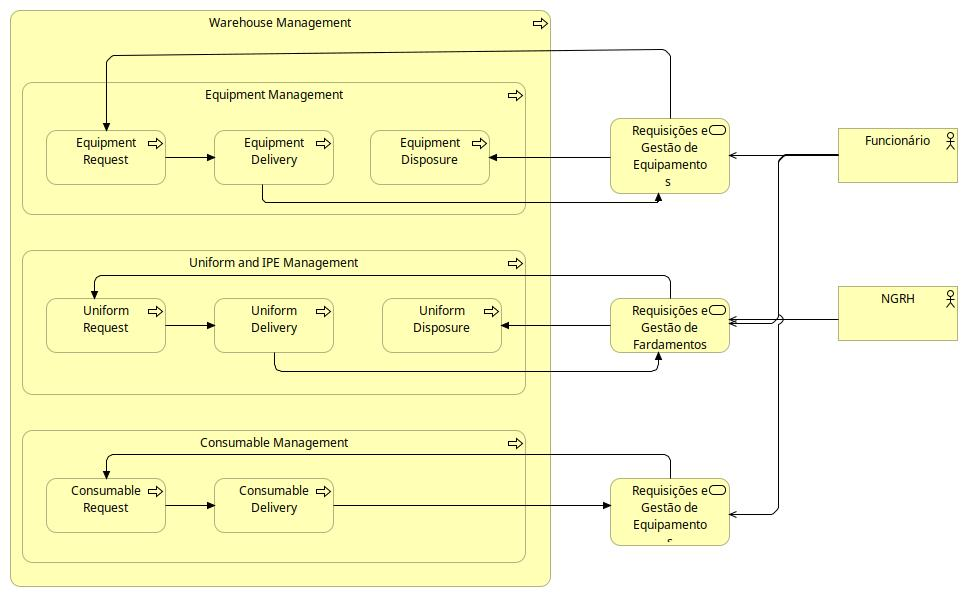
\includegraphics[width=0.8\textwidth]{Q4a - Gestão de Armazém.jpg}
        \caption{Relação entre serviços e processos de negócio – Gestão de Armazém}
        \label{fig:q4-armazem}
    \end{figure}

    \begin{figure}[H]
        \centering
        \includegraphics[width=0.8\textwidth]{Q4b - Gestão de Frota.jpg}
        \caption{Relação entre serviços e processos de negócio – Gestão de Frota}
        \label{fig:q4-frota}
    \end{figure}

    \begin{figure}[H]
        \centering
        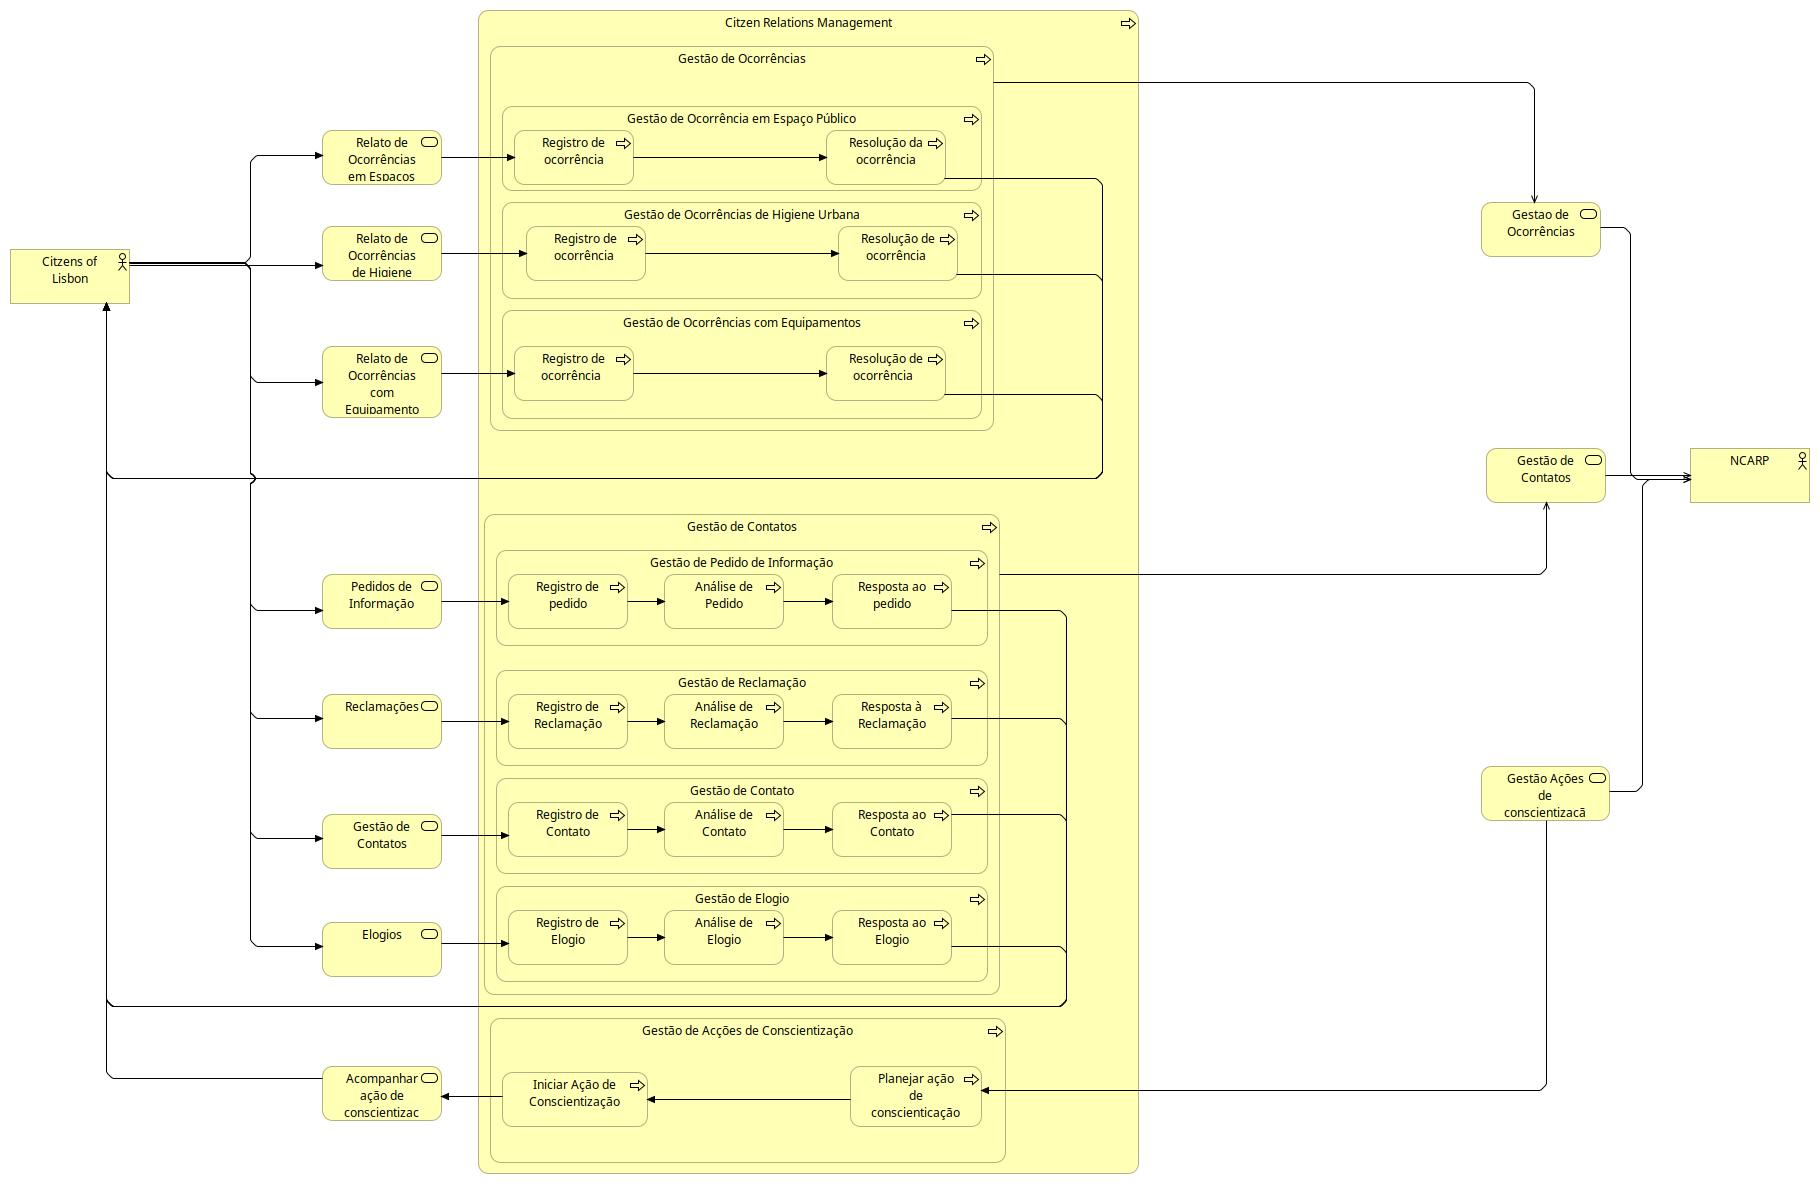
\includegraphics[width=0.8\textwidth]{Q4c - Gestão das Relações com cidadão.jpg}
        \caption{Relação entre serviços e processos de negócio – Gestão das Relações com o Cidadão}
        \label{fig:q4-cidadao}
    \end{figure}

    \begin{figure}[H]
        \centering
        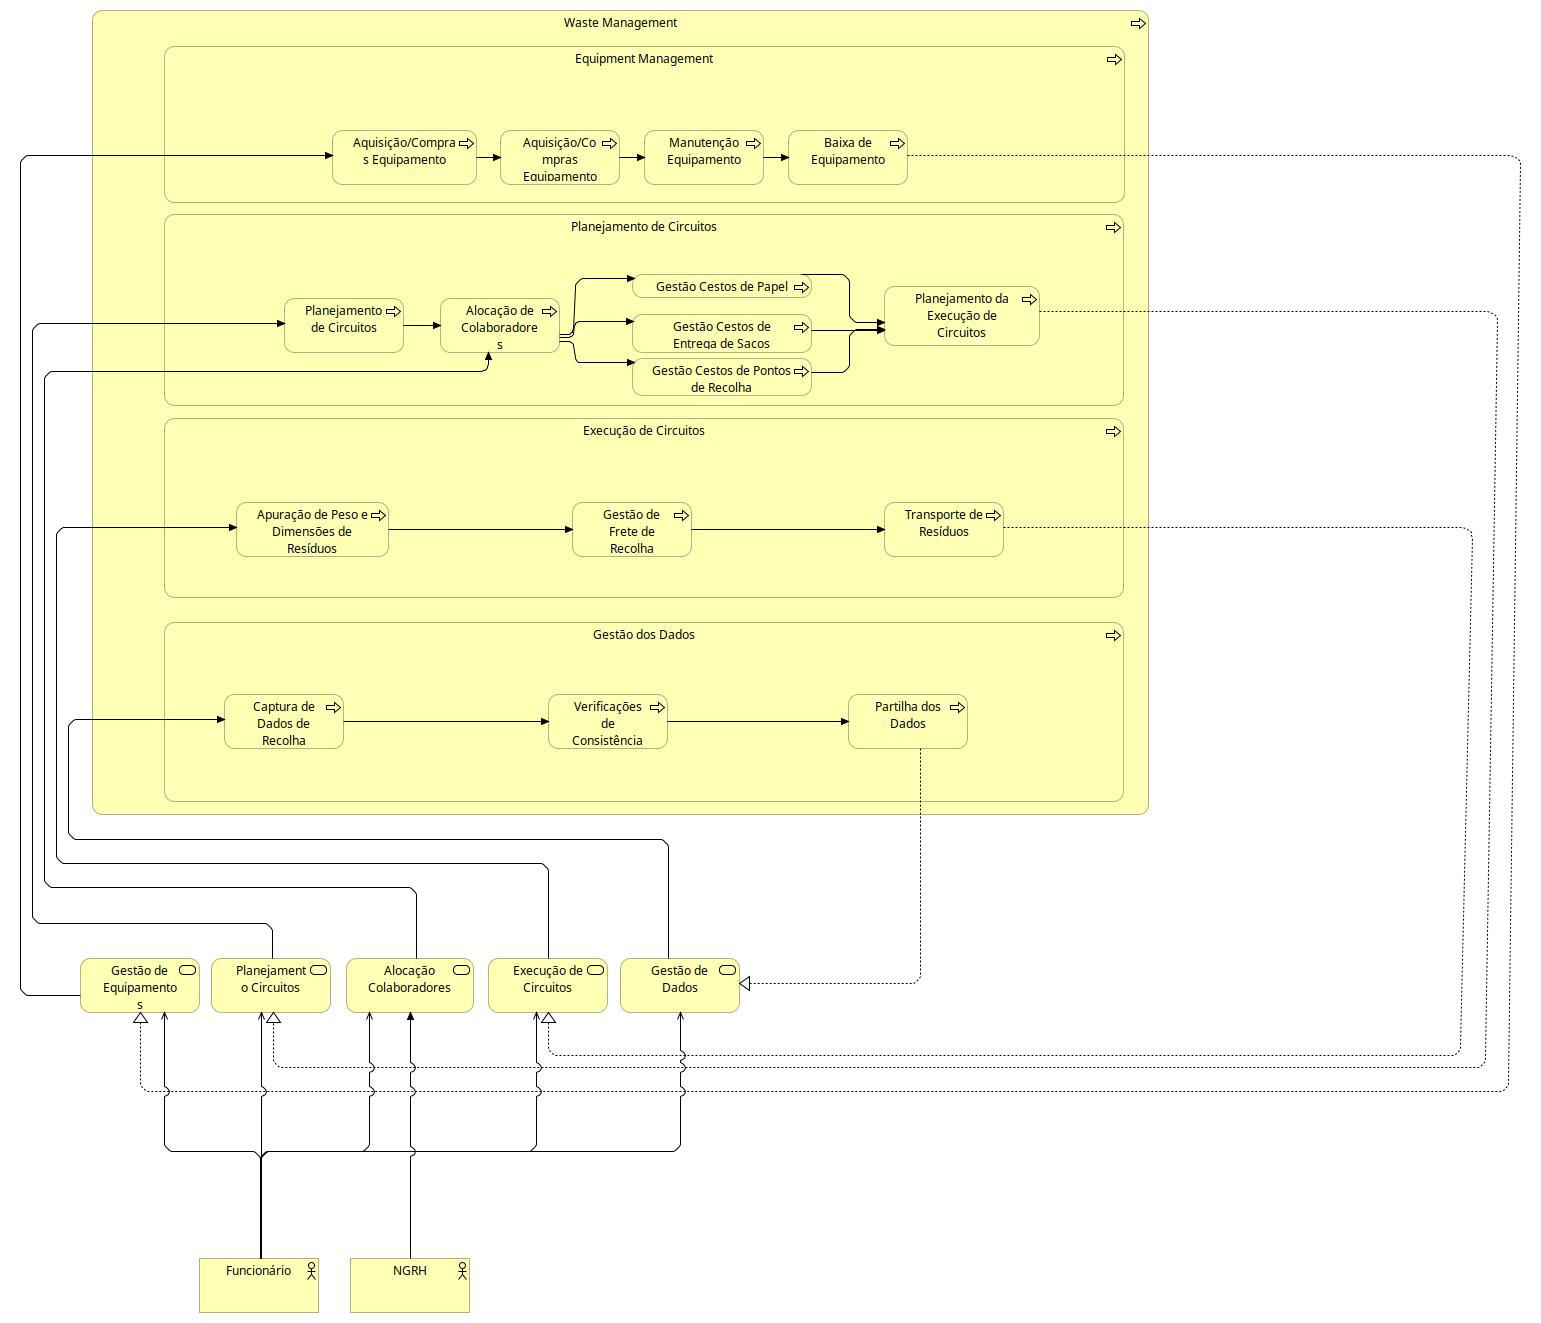
\includegraphics[width=0.8\textwidth]{Q4d - Gestão de Resíduos.jpg}
        \caption{Relação entre serviços e processos de negócio – Gestão de Resíduos}
        \label{fig:q4-residuos}
    \end{figure}

    \begin{figure}[H]
        \centering
        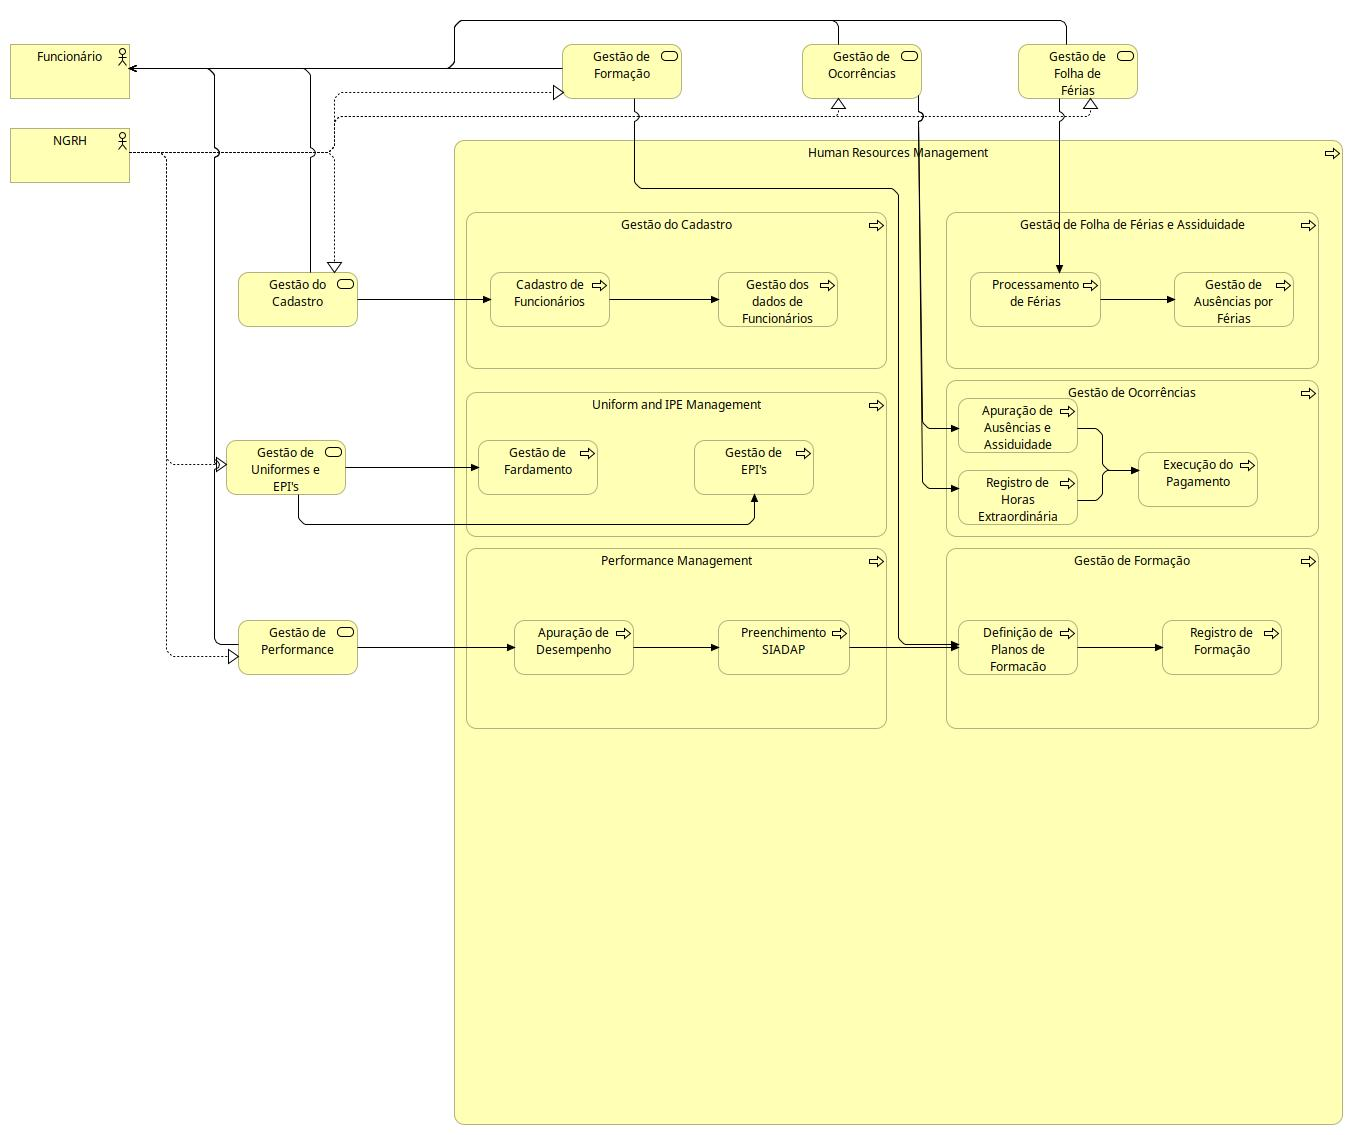
\includegraphics[width=0.8\textwidth]{Q4e - Recursos Humanos.jpg}
        \caption{Relação entre serviços e processos de negócio – Recursos Humanos}
        \label{fig:q4-rh}
    \end{figure}

    \textbf{Análise:} Foi reforçada a articulação entre processos e a exposição dos serviços, corrigindo o reduzido número de processos iniciais e melhorando a legibilidade dos diagramas, tal como sugerido em feedback. Agora, é visível a dependência e contributo de cada processo para a prestação de serviços DMHU.


    \section*{Questão 5 – Especificação de Alto Nível dos Processos de Negócio (Black-box)}
    \addcontentsline{toc}{section}{Q5 – Especificação de Alto Nível dos Processos de Negócio}
    Os diagramas seguintes representam, ao nível mais abstrato, a configuração dos meta-processos chave em cada área funcional. Foi feito um esforço de simplificação para centrar nos processos estruturantes, garantindo clareza de fronteiras (“black-box”).

    \begin{figure}[H]
        \centering
        \includegraphics[width=0.85\textwidth]{Q5a - Recolha de Resíduos.jpg}
        \caption{Processo de Negócio – Recolha de Resíduos}
        \label{fig:q5-residuos}
    \end{figure}

    \begin{figure}[H]
        \centering
        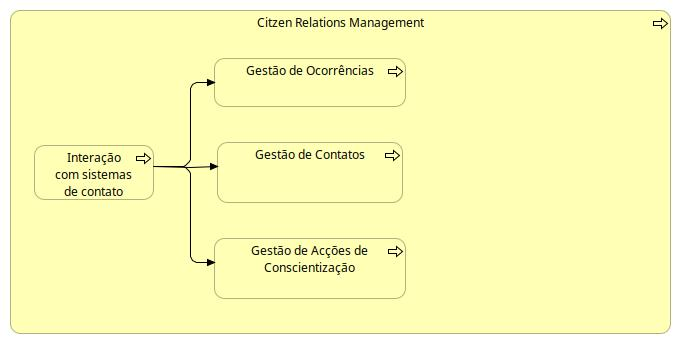
\includegraphics[width=0.85\textwidth]{Q5b - Relações com Cidadão.jpg}
        \caption{Processo de Negócio – Relações com Cidadão}
        \label{fig:q5-cidadao}
    \end{figure}

    \begin{figure}[H]
        \centering
        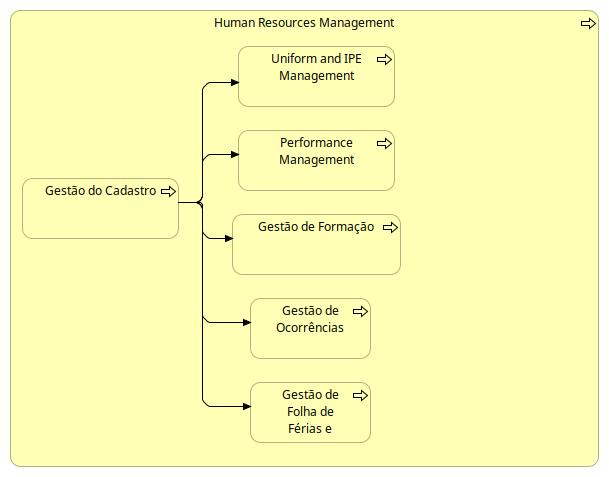
\includegraphics[width=0.85\textwidth]{Q5c - Recursos Humanos.jpg}
        \caption{Processo de Negócio – Recursos Humanos}
        \label{fig:q5-rh}
    \end{figure}

    \begin{figure}[H]
        \centering
        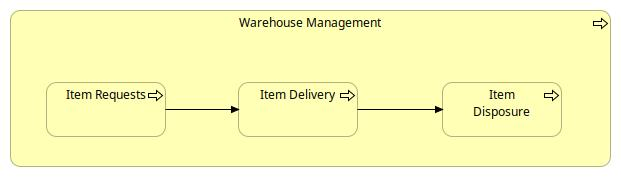
\includegraphics[width=0.85\textwidth]{Q5d - Gestão de Armazém.jpg}
        \caption{Processo de Negócio – Gestão de Armazém}
        \label{fig:q5-armazem}
    \end{figure}

    \begin{figure}[H]
        \centering
        \includegraphics[width=0.85\textwidth]{Q5e - Gestão de Frota.jpg}
        \caption{Processo de Negócio – Gestão de Frota}
        \label{fig:q5-frota}
    \end{figure}

    \textbf{Nota:} Este modelo foi refeito para garantir clareza de fronteiras de processos e aumentar a legibilidade, respondendo à crítica de complexidade excessiva do diagrama inicial.


    \section*{Questão 6 – Especificação Operacional Interna dos Processos (White-box)}
    \addcontentsline{toc}{section}{Q6 - Especificação Operacional Interna dos Processos}

    Cada um dos diagramas seguintes detalha a operação interna dos processos mais relevantes, mapeando subprocessos e interligações. Em resultado do feedback, foi reforçada a ligação entre subprocessos e a identificação dos principais fluxos internos.

    \begin{figure}[H]
        \centering
        \includegraphics[width=0.85\textwidth]{Q6a - Recolha de Resíduos.jpg}
        \caption{Detalhe Operacional – Recolha de Resíduos}
        \label{fig:q6-residuos}
    \end{figure}

    \begin{figure}[H]
        \centering
        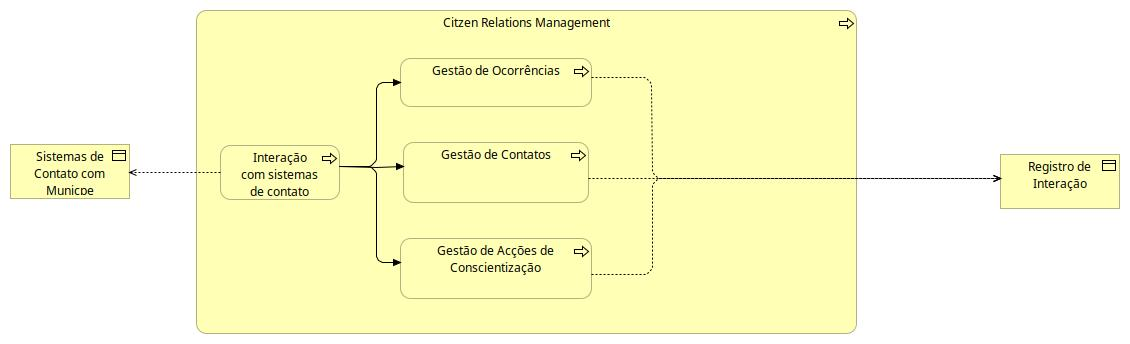
\includegraphics[width=0.85\textwidth]{Q6b - Relações com Cidadão.jpg}
        \caption{Detalhe Operacional – Relações com Cidadão}
        \label{fig:q6-cidadao}
    \end{figure}

    \begin{figure}[H]
        \centering
        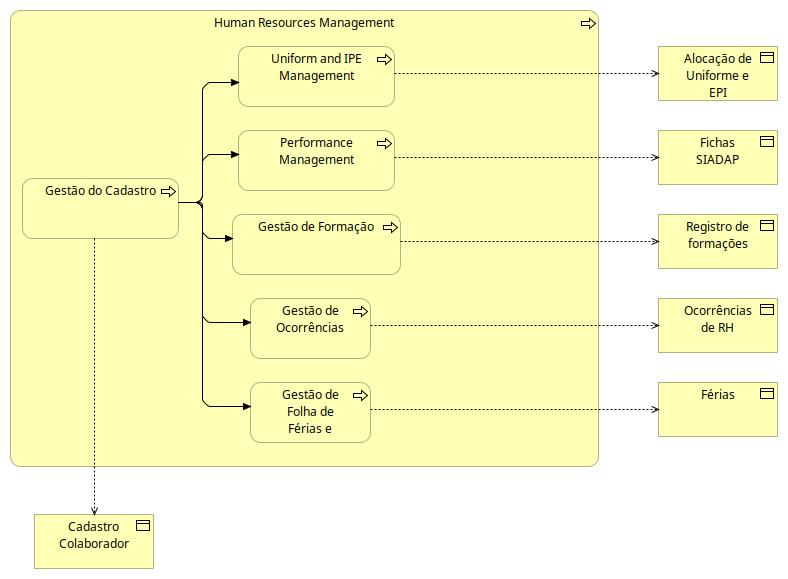
\includegraphics[width=0.85\textwidth]{Q6c - Recursos Humanos.jpg}
        \caption{Detalhe Operacional – Recursos Humanos}
        \label{fig:q6-rh}
    \end{figure}

    \begin{figure}[H]
        \centering
        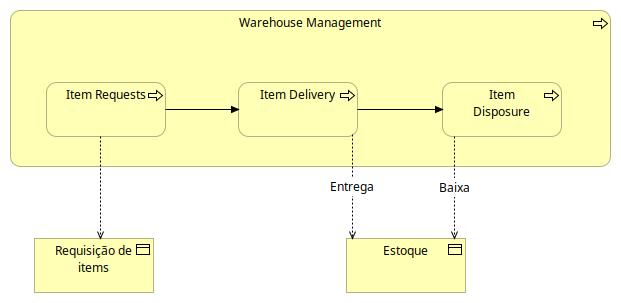
\includegraphics[width=0.85\textwidth]{Q6d - Gestão de Armazém.jpg}
        \caption{Detalhe Operacional – Gestão de Armazém}
        \label{fig:q6-armazem}
    \end{figure}

    \begin{figure}[H]
        \centering
        \includegraphics[width=0.85\textwidth]{Q6e - Gestão de Frota.jpg}
        \caption{Detalhe Operacional – Gestão de Frota}
        \label{fig:q6-frota}
    \end{figure}

    \textbf{Nota:} Estes diagramas apresentam agora uma visão mais realista das relações entre subprocessos e os fluxos de trabalho, em resposta ao feedback relativo à pouca interligação dos processos apresentados inicialmente.


    \section*{Questão 7 – Entidades Informacionais e Classificação Inmon}
    \addcontentsline{toc}{section}{Q7 - Entidades de Informação da DMHU}

    Em resposta ao feedback anterior e considerando a abrangência dos processos da Direção Municipal de Higiene Urbana (DMHU), procedeu-se à identificação exaustiva das entidades informacionais críticas à operação e gestão do serviço. Cada entidade foi classificada segundo o modelo de William H. Inmon — distinguindo-se agora claramente a sua origem (primitiva ou derivada), a sua dimensão temporal (histórica, projetada, referencial) e o respetivo regime de acesso (público/privado).

    Esta abordagem tripla visa garantir rastreabilidade, robustez e preparação para integração com soluções avançadas de análise e governação de dados. A Tabela~\ref{tab:inmon} apresenta a classificação detalhada, que abrange todas as áreas operacionais representadas nos modelos de domínio da Q8 e corrige as lacunas identificadas nas versões anteriores do trabalho.

    \renewcommand{\arraystretch}{1.3}
    \begin{longtable}{|p{6cm}|p{7cm}|}
        \caption{Classificação Inmon das entidades de informação da DMHU}
        \label{tab:inmon} \\
        \hline
        \textbf{Entidade Informacional}          & \textbf{Classificação Inmon}    \\
        \hline
        \endfirsthead
        \hline
        \textbf{Entidade Informacional}          & \textbf{Classificação Inmon}    \\
        \hline
        \endhead
        \hline
        \endfoot


        Cidadão                                  & Primitiva, Histórica, Pública   \\
        Ocorrência                               & Primitiva, Histórica, Pública   \\
        Pedido de Assistência                    & Derivada, Histórica, Pública    \\
        Folha de Inquérito                       & Derivada, Histórica, Privada    \\
        Resposta de Serviço                      & Derivada, Histórica, Privada    \\
        Resposta Associada                       & Derivada, Histórica, Privada    \\
        Endereço                                 & Primitiva, Histórica, Pública   \\
        Equipamento de Deposição                 & Primitiva, Histórica, Pública   \\
        Local de Contentor                       & Primitiva, Projetada, Pública   \\
        Circuito de Recolha                      & Primitiva, Projetada, Pública   \\
        PRS (Ponto de Recolha Seletiva)          & Primitiva, Histórica, Pública   \\
        Área de Apoio                            & Primitiva, Projetada, Privada   \\
        Local de Descarga                        & Primitiva, Projetada, Pública   \\
        Requisição ao Armazém                    & Derivada, Histórica, Privada    \\
        Bem Móvel / Stock                        & Primitiva, Histórica, Privada   \\
        Funcionário (Colaborador)                & Primitiva, Histórica, Privada   \\
        Frequência/Formação                      & Derivada, Histórica, Privada    \\
        Curso de Formação                        & Primitiva, Projetada, Privada   \\
        Uniforme                                 & Primitiva, Projetada, Privada   \\
        Equipamento de Proteção Individual       & Primitiva, Projetada, Privada   \\
        Equipamento (Máquinas)                   & Primitiva, Histórica, Privada   \\
        Veículo                                  & Primitiva, Histórica, Privada   \\
        Movimento de Equipamento                 & Derivada, Histórica, Privada    \\
        Garage                                   & Primitiva, Projetada, Privada   \\
        Tipo de Máquina                          & Primitiva, Referencial, Pública \\
        Oficina                                  & Primitiva, Projetada, Privada   \\
        Plano de Manutenção                      & Derivada, Projetada, Privada    \\
        Inspeção                                 & Derivada, Histórica, Privada    \\
        Evento (ação pública)                    & Derivada, Histórica, Pública    \\
        Reclamação                               & Primitiva, Histórica, Pública   \\
        Sugestão                                 & Primitiva, Histórica, Pública   \\
        Pedido de Recolha Volumosa               & Derivada, Histórica, Pública    \\
        Pedido de Controlo de Pragas             & Derivada, Histórica, Pública    \\
        Pedido de Contentor                      & Derivada, Histórica, Pública    \\
        Pedido de Intervenção                    & Derivada, Histórica, Pública    \\
        Pedido de Evento                         & Derivada, Histórica, Pública    \\
        Avaliação de Desempenho                  & Derivada, Histórica, Privada    \\
        Atestado de Aptidão Médica               & Primitiva, Histórica, Privada   \\
        Acidente de Trabalho                     & Primitiva, Histórica, Privada   \\
        Ausência/Assiduidade                     & Derivada, Histórica, Privada    \\
        Registo de Frequência (Relógio de Ponto) & Primitiva, Histórica, Privada   \\
        Responsável de Circuito/Operação         & Primitiva, Histórica, Privada   \\

    \end{longtable}

    \textbf{Nota:} Com esta revisão, foram endereçados os principais problemas apontados no feedback, nomeadamente a falta de entidades, a classificação imprópria e a ausência de correspondência com os modelos de domínio das várias áreas funcionais da DMHU.



    \newpage
    \section*{Questão 8 – Modelo de Domínio das Entidades Informacionais}
    \addcontentsline{toc}{section}{Q8 – Modelo de Domínio das Entidades Informacionais}

    Nesta secção, são apresentados os modelos de domínio por área funcional. Foram corrigidas as classificações de acordo com a tipologia de Inmon: \textit{Primitiva/Derivada}, \textit{Histórica/Projetada}, \textit{Pública/Privada}. Cada diagrama é acompanhado por uma descrição textual que detalha as principais entidades e relações modeladas.

    \begin{figure}[H]
        \centering
        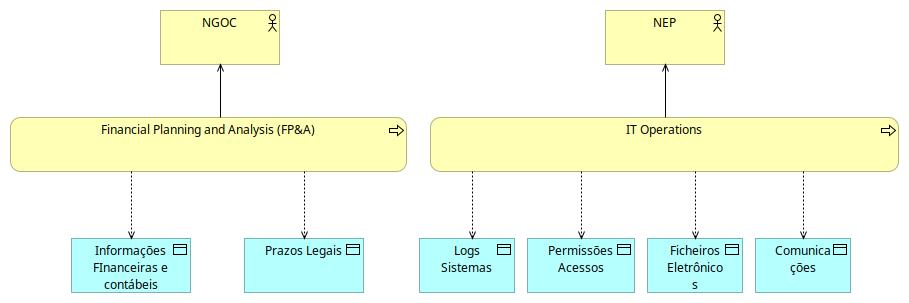
\includegraphics[width=0.9\textwidth]{Q8 - Domain Model For Information Entities - Admin Ops.jpg}
        \caption{Modelo de Domínio – Administração Operacional}
        \label{fig:q8-adminops}
    \end{figure}

    \textbf{Análise:} O modelo inclui entidades como \textit{Logs de Sistema}, \textit{Permissões de Acesso}, e \textit{Ficheiros Electrónicos}, cruciais para auditoria e compliance. Todas estas entidades foram classificadas como \textit{Primitivas} e \textit{Históricas}, sendo a maioria de \textit{acesso privado}.

    \begin{figure}[H]
        \centering
        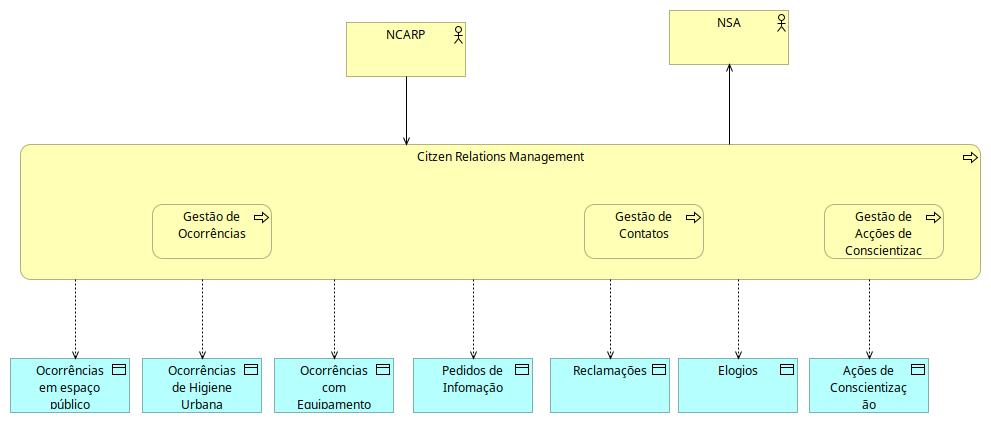
\includegraphics[width=0.9\textwidth]{Q8 - Domain Model For Information Entities - Citzen Relationship Management.jpg}
        \caption{Modelo de Domínio – Gestão das Relações com o Cidadão}
        \label{fig:q8-cidadao}
    \end{figure}

    \textbf{Análise:} A gestão das relações com o cidadão contempla entidades como \textit{Ocorrência}, \textit{Pedido de Intervenção}, \textit{Resposta}, e \textit{Endereço}. A \textit{Ocorrência} é uma entidade primitiva, pública e histórica, dado que se origina da participação do cidadão e permanece para efeitos de análise futura.

    \begin{figure}[H]
        \centering
        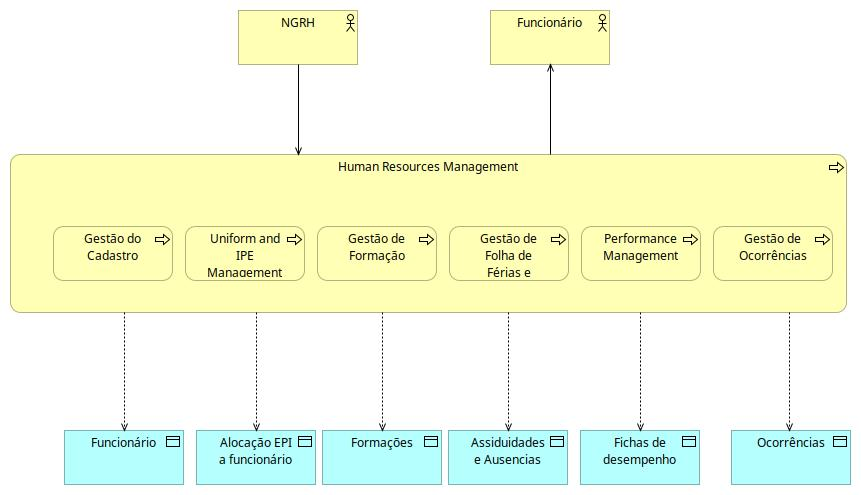
\includegraphics[width=0.9\textwidth]{Q8 - Domain Model For Information Entities - Human Ressources Management.jpg}
        \caption{Modelo de Domínio – Recursos Humanos}
        \label{fig:q8-rh}
    \end{figure}

    \textbf{Análise:} No contexto de RH, destacam-se entidades como \textit{Funcionário}, \textit{Formação}, \textit{Incidente}, e \textit{Avaliação de Desempenho}. Os \textit{Funcionários} são entidades primitivas, privadas e projetadas; enquanto que os registos de formação e avaliação são históricos e derivam da atividade do trabalhador.

    \begin{figure}[H]
        \centering
        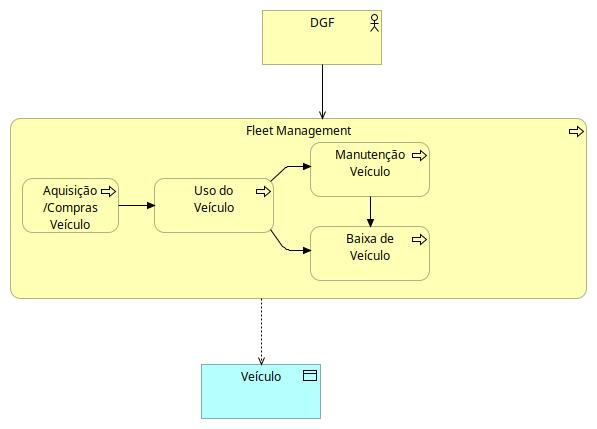
\includegraphics[width=0.9\textwidth]{Q8 - Domain Model For Information Entities - Fleet Management.jpg}
        \caption{Modelo de Domínio – Gestão de Frota}
        \label{fig:q8-frota}
    \end{figure}

    \textbf{Análise:} A frota municipal é composta por \textit{Viaturas}, \textit{Ordens de Trabalho}, \textit{Equipamentos}, entre outros. As viaturas são registadas como ativos móveis e as ordens de trabalho são documentos derivados, usados para manutenção e histórico de atividade.

    \begin{figure}[H]
        \centering
        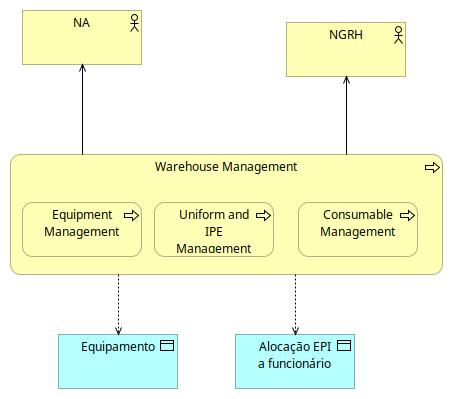
\includegraphics[width=0.9\textwidth]{Q8 - Domain Model For Information Entities - Warehouse Management.jpg}
        \caption{Modelo de Domínio – Gestão de Armazém}
        \label{fig:q8-armazem}
    \end{figure}

    \textbf{Análise:} O armazém gere entidades como \textit{Pedido de Requisição}, \textit{Uniformes}, \textit{Stock}, e \textit{Funcionário}. Os \textit{Uniformes} são elementos de inventário com tempo de vida útil, sendo ligados a períodos de entrega e consumo projetado.

    \begin{figure}[H]
        \centering
        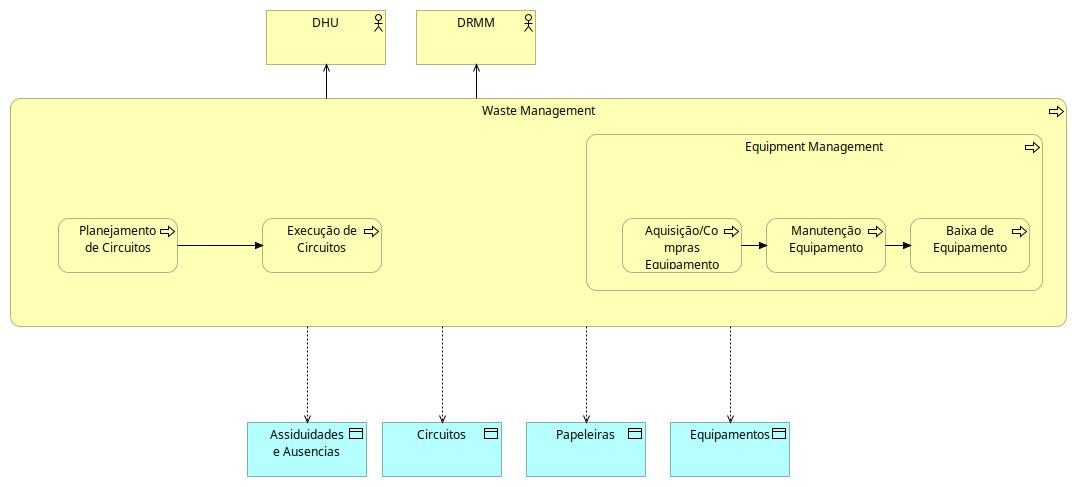
\includegraphics[width=0.9\textwidth]{Q8 - Domain Model For Information Entities - Waste Management.jpg}
        \caption{Modelo de Domínio – Gestão de Resíduos}
        \label{fig:q8-residuos}
    \end{figure}

    \textbf{Análise:} Este modelo contempla \textit{Circuitos}, \textit{Pontos de Recolha Seletiva}, \textit{Equipamento de Deposição}, e \textit{Requisições de Serviço}. Os pontos de recolha são elementos primitivos e públicos, já os circuitos são derivados de múltiplas entidades para otimização de rotas.

    \begin{figure}[H]
        \centering
        \includegraphics[width=0.9\textwidth]{Q8 - Domain Model For Information Entities - Miscelânea.jpg}
        \caption{Modelo de Domínio – Miscelânea}
        \label{fig:q8-miscelanea}
    \end{figure}

    \textbf{Análise:} Incluem-se nesta categoria entidades como \textit{Eventos}, \textit{Ações de Sensibilização}, \textit{Animais Apreendidos}, e \textit{Pontos de Interesse}. Estas entidades cobrem áreas complementares, geralmente com origem externa, sendo na maioria públicas e projetadas.

    \begin{figure}[H]
        \centering
        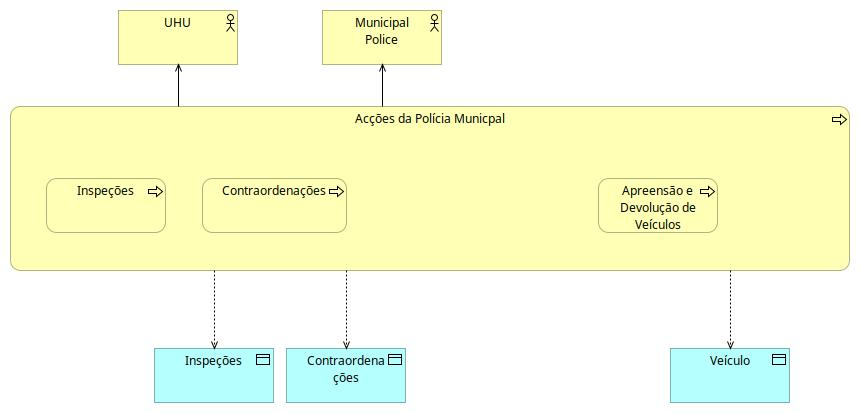
\includegraphics[width=0.9\textwidth]{Q8 - Domain Model For Information Entities - Municipal Police.jpg}
        \caption{Modelo de Domínio – Polícia Municipal}
        \label{fig:q8-pm}
    \end{figure}

    \textbf{Análise:} As entidades deste modelo dizem respeito à fiscalização: \textit{Infrações}, \textit{Veículos Apreendidos}, \textit{Registos de Inspeção}. As infrações são públicas e históricas, enquanto os veículos e relatórios podem ter restrições de acesso, sendo classificados como privados.

    \section*{Questão 9 – Arquitetura Aplicacional AS-IS}
    \addcontentsline{toc}{section}{Q9 - Application Structure as-is}

    O diagrama seguinte apresenta a arquitetura das aplicações atualmente em funcionamento na DMHU, segmentadas por domínio funcional (Relação com o Cidadão, Recursos Humanos, Frota, Armazém, etc.). Após revisão, as ligações entre aplicações e processos de negócio foram clarificadas, distinguindo interfaces, serviços e sistemas de backend.

    \begin{figure}[H]
        \centering
        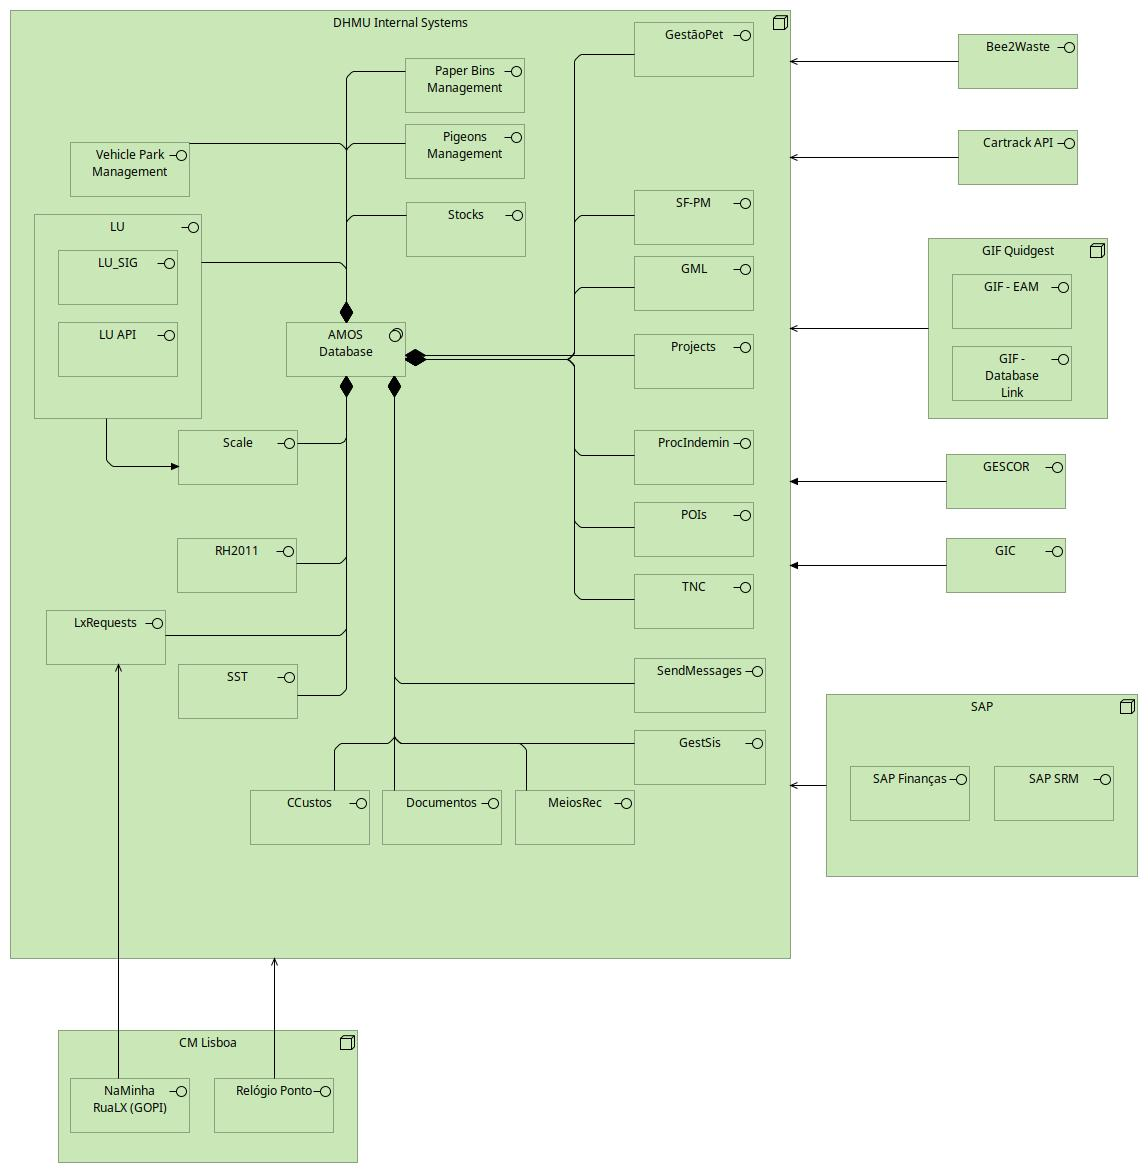
\includegraphics[width=0.95\textwidth]{Q9 - Application Structure as Is - Application Structure.jpg}
        \caption{Estrutura aplicacional AS-IS da DMHU}
        \label{fig:q9-app-structure}
    \end{figure}

    \textbf{Análise:} Foram corrigidas ambiguidades e clarificadas as relações entre módulos e aplicações, colmatando erros de sobreposição de serviços, interfaces e camadas tecnológicas.

    \section*{Questão 10 – Utilização das Aplicações AS-IS}
    \addcontentsline{toc}{section}{Q10 - Application Usage as-is}

    Segue-se a caracterização do uso das aplicações por área funcional, explicitando como cada aplicação suporta os processos de negócio. Esta análise encontra-se distribuída por vários diagramas:

    \begin{figure}[H]
        \centering
        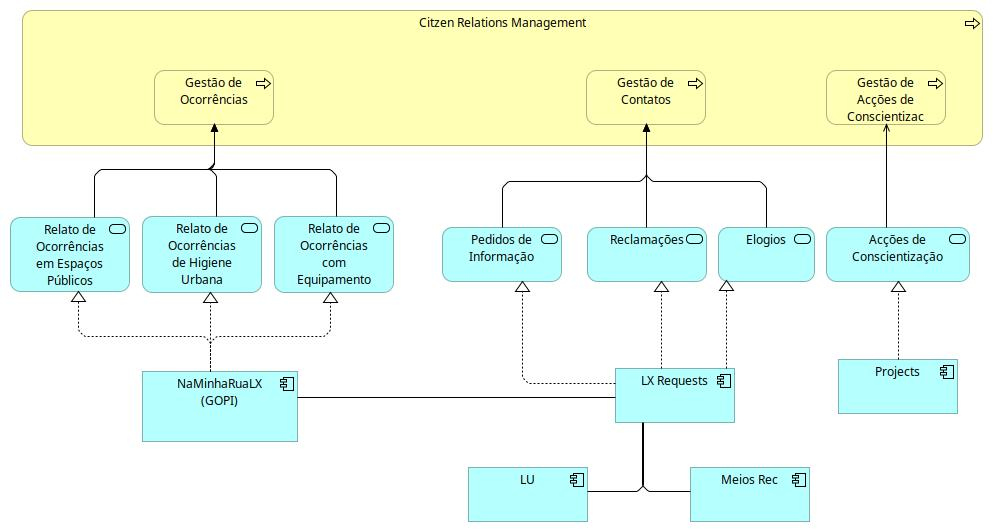
\includegraphics[width=0.47\textwidth]{Q10 - Application Usage - Citzen Relations Management.jpg}
        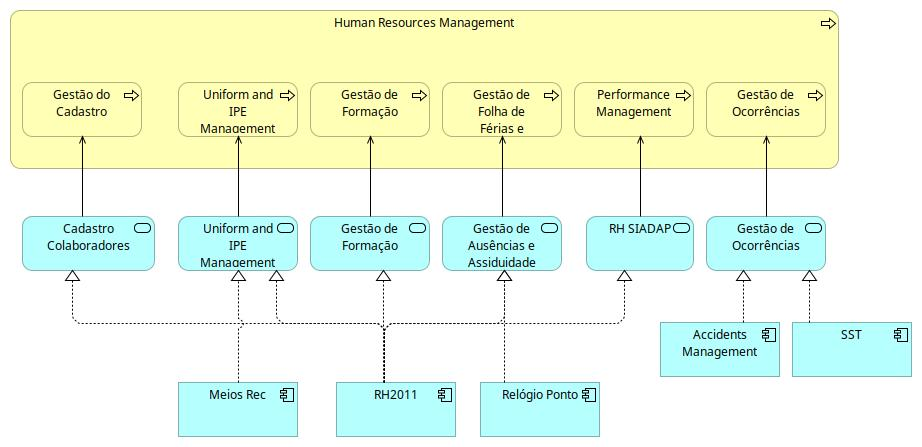
\includegraphics[width=0.47\textwidth]{Q10 - Application Usage - Human Ressources Management.jpg}
        \caption{Utilização das aplicações – Relação com o Cidadão e Recursos Humanos}
        \label{fig:q10-usage-cidadao-rh}
    \end{figure}

    \begin{figure}[H]
        \centering
        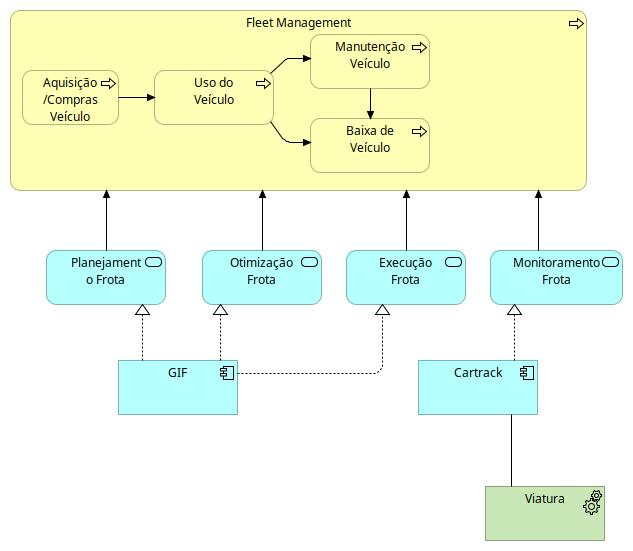
\includegraphics[width=0.47\textwidth]{Q10 - Application Usage - Fleet Management.jpg}
        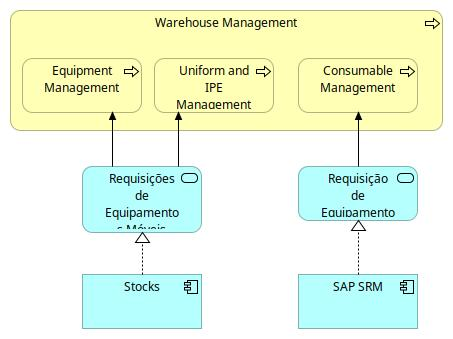
\includegraphics[width=0.47\textwidth]{Q10 - Application Usage - Warehouse Management.jpg}
        \caption{Utilização das aplicações – Gestão de Frota e Armazém}
        \label{fig:q10-usage-frota-armazem}
    \end{figure}

    \begin{figure}[H]
        \centering
        \includegraphics[width=0.47\textwidth]{Q10 - Application Usage - Miscelânea.jpg}
        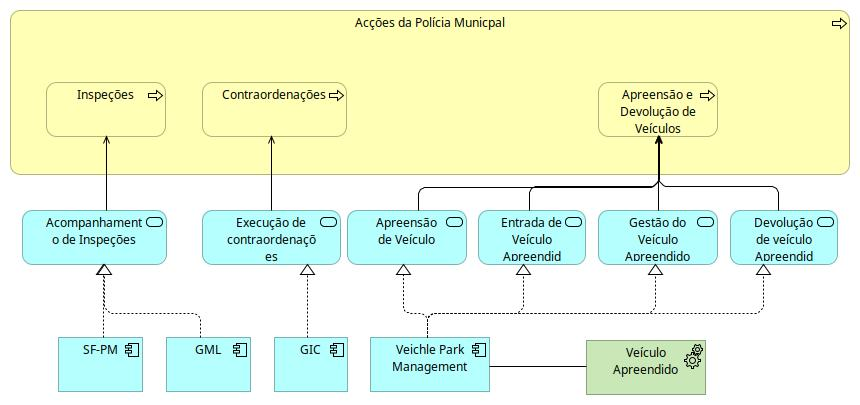
\includegraphics[width=0.47\textwidth]{Q10 - Application Usage - Municipal Police.jpg}
        \caption{Utilização das aplicações – Miscelânea e Polícia Municipal}
        \label{fig:q10-usage-misc-pm}
    \end{figure}

    \textbf{Nota:} O novo mapeamento reforça a clareza entre aplicações, elimina interfaces redundantes e corrige inconsistências apontadas no feedback.

    \section*{Questão 11 – Infraestrutura de Processamento AS-IS}
    \addcontentsline{toc}{section}{Q11 - Processing Infrastructure as-is}

    O diagrama seguinte detalha a infraestrutura de processamento existente, incluindo servidores físicos e virtuais, agrupamentos de aplicações e camadas de suporte.

    \begin{figure}[H]
        \centering
        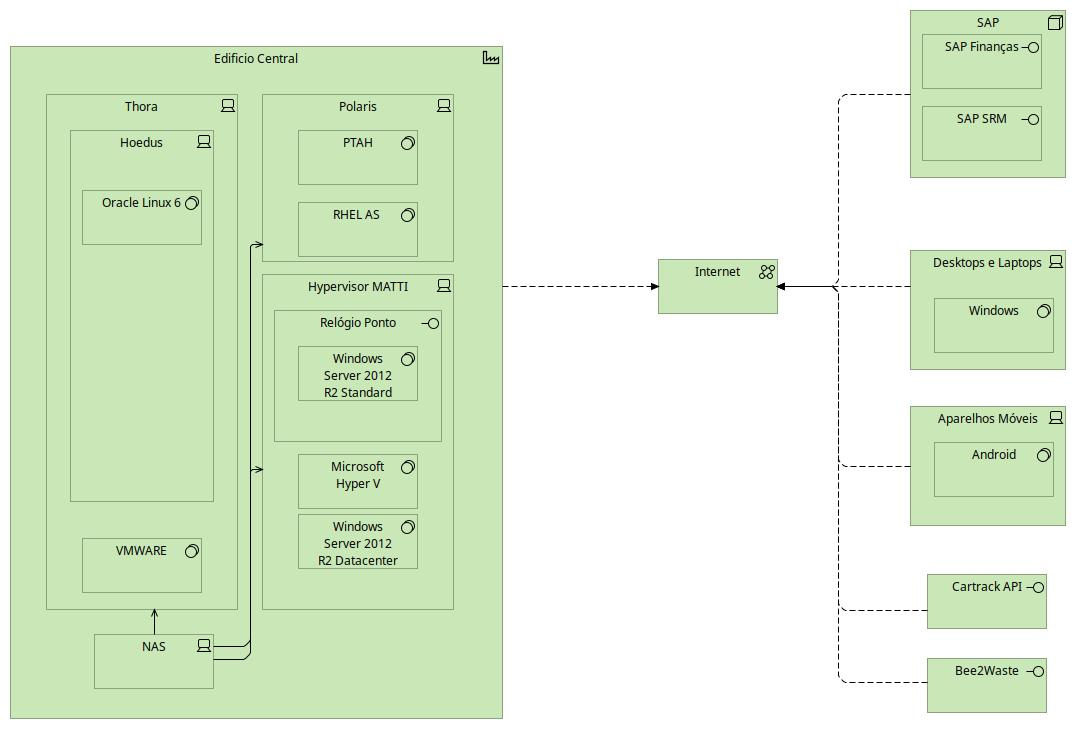
\includegraphics[width=0.95\textwidth]{Q11 - Processing Infraestructure As-Is.jpg}
        \caption{Infraestrutura de processamento AS-IS da DMHU}
        \label{fig:q11-processing}
    \end{figure}

    \textbf{Nota:} Foram explicitadas dependências críticas, agrupamentos lógicos e tecnologias-chave, melhorando a legibilidade da infraestrutura, conforme sugerido pelo professor.

    \section*{Questão 12 – Infraestrutura de Armazenamento AS-IS}
    \addcontentsline{toc}{section}{Q12 - Storage Infrastructure as-is}

    O seguinte diagrama evidencia os equipamentos de armazenamento e as bases de dados que suportam o funcionamento das aplicações DMHU.

    \begin{figure}[H]
        \centering
        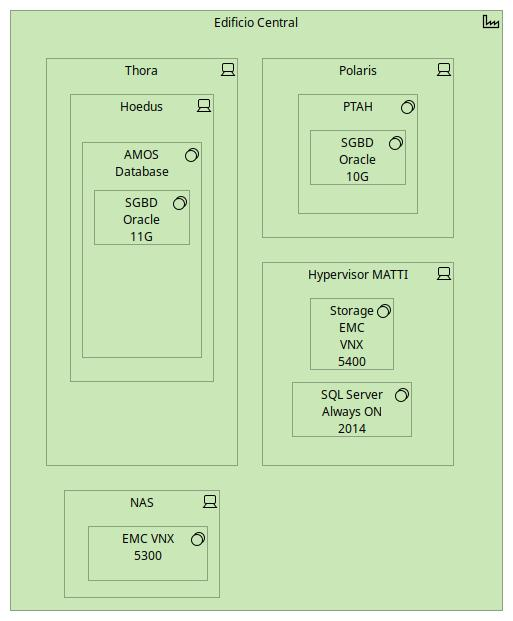
\includegraphics[width=0.95\textwidth]{Q12 - Storage Infraestructure As-Is.jpg}
        \caption{Infraestrutura de armazenamento AS-IS da DMHU}
        \label{fig:q12-storage}
    \end{figure}

    Esta abordagem permite:
    \begin{itemize}
        \item Identificar dependências críticas entre aplicações e infraestruturas físicas;
        \item Detetar pontos de concentração de risco (single points of failure) ao nível do armazenamento;
        \item Suportar auditorias, gestão de backups e planeamento de migração.
    \end{itemize}

    Esta estruturação não só suporta o funcionamento eficiente dos sistemas atuais, como é crítica para o sucesso de futuras migrações, auditorias e planos de disaster recovery.

    \section*{Q13 - Matriz CRUD entre Entidades e Processos}
    \addcontentsline{toc}{section}{Q13 - Matriz CRUD entre Entidades e Processos}

    A matriz CRUD (ver anexo \textit{matriz\_crudQ13\_Q14.ods}) relaciona processos de negócio e entidades
    informacionais. A sua análise detalhada permite identificar zonas de risco e de melhoria, em particular:

    \begin{itemize}
        \item \textbf{Silos funcionais:} Exemplo concreto – a entidade \textit{Formação} é gerida exclusivamente pelo processo “Gestão de Formação” e pela respetiva aplicação de RH. Não existe integração direta com outros processos que poderiam beneficiar desta informação, como a Avaliação de Desempenho ou a Gestão de Equipamentos, criando um silo de informação.
        \item \textbf{Sobreposições funcionais:} Exemplo – a entidade \textit{Ocorrência} é criada e lida tanto pelos processos de Gestão de Relação com o Cidadão como pelos processos de Gestão de Resíduos. Estes processos utilizam aplicações distintas, o que pode originar duplicação, inconsistência ou atraso na partilha de dados.
        \item \textbf{Redundâncias e pontos críticos:} A entidade \textit{Equipamento} é atualizada tanto pela Gestão de Frota como pelo Armazém. Sem mecanismos robustos de sincronização, existe risco de conflito ou perda de rastreabilidade.
    \end{itemize}

    Estes exemplos concretos, identificados na matriz CRUD, fundamentam a necessidade de integração mais eficiente e de uma governação de dados transversal a toda a DMHU.

    Recomenda-se a implementação de políticas de governação de dados que permitam identificar, monitorizar e atuar preventivamente sobre potenciais conflitos, silos e redundâncias.

    \section*{Q14 - Matriz CRUD com Aplicações e Dependências (BSP)}
    \addcontentsline{toc}{section}{Q14 - Matriz CRUD com Aplicações e Dependências (BSP)}

    A Figura~\ref{fig:q14-domains} apresenta os domínios informacionais e entidades por área funcional, complementada pela matriz CRUD/anexo BSP.

    \begin{figure}[H]
        \centering
        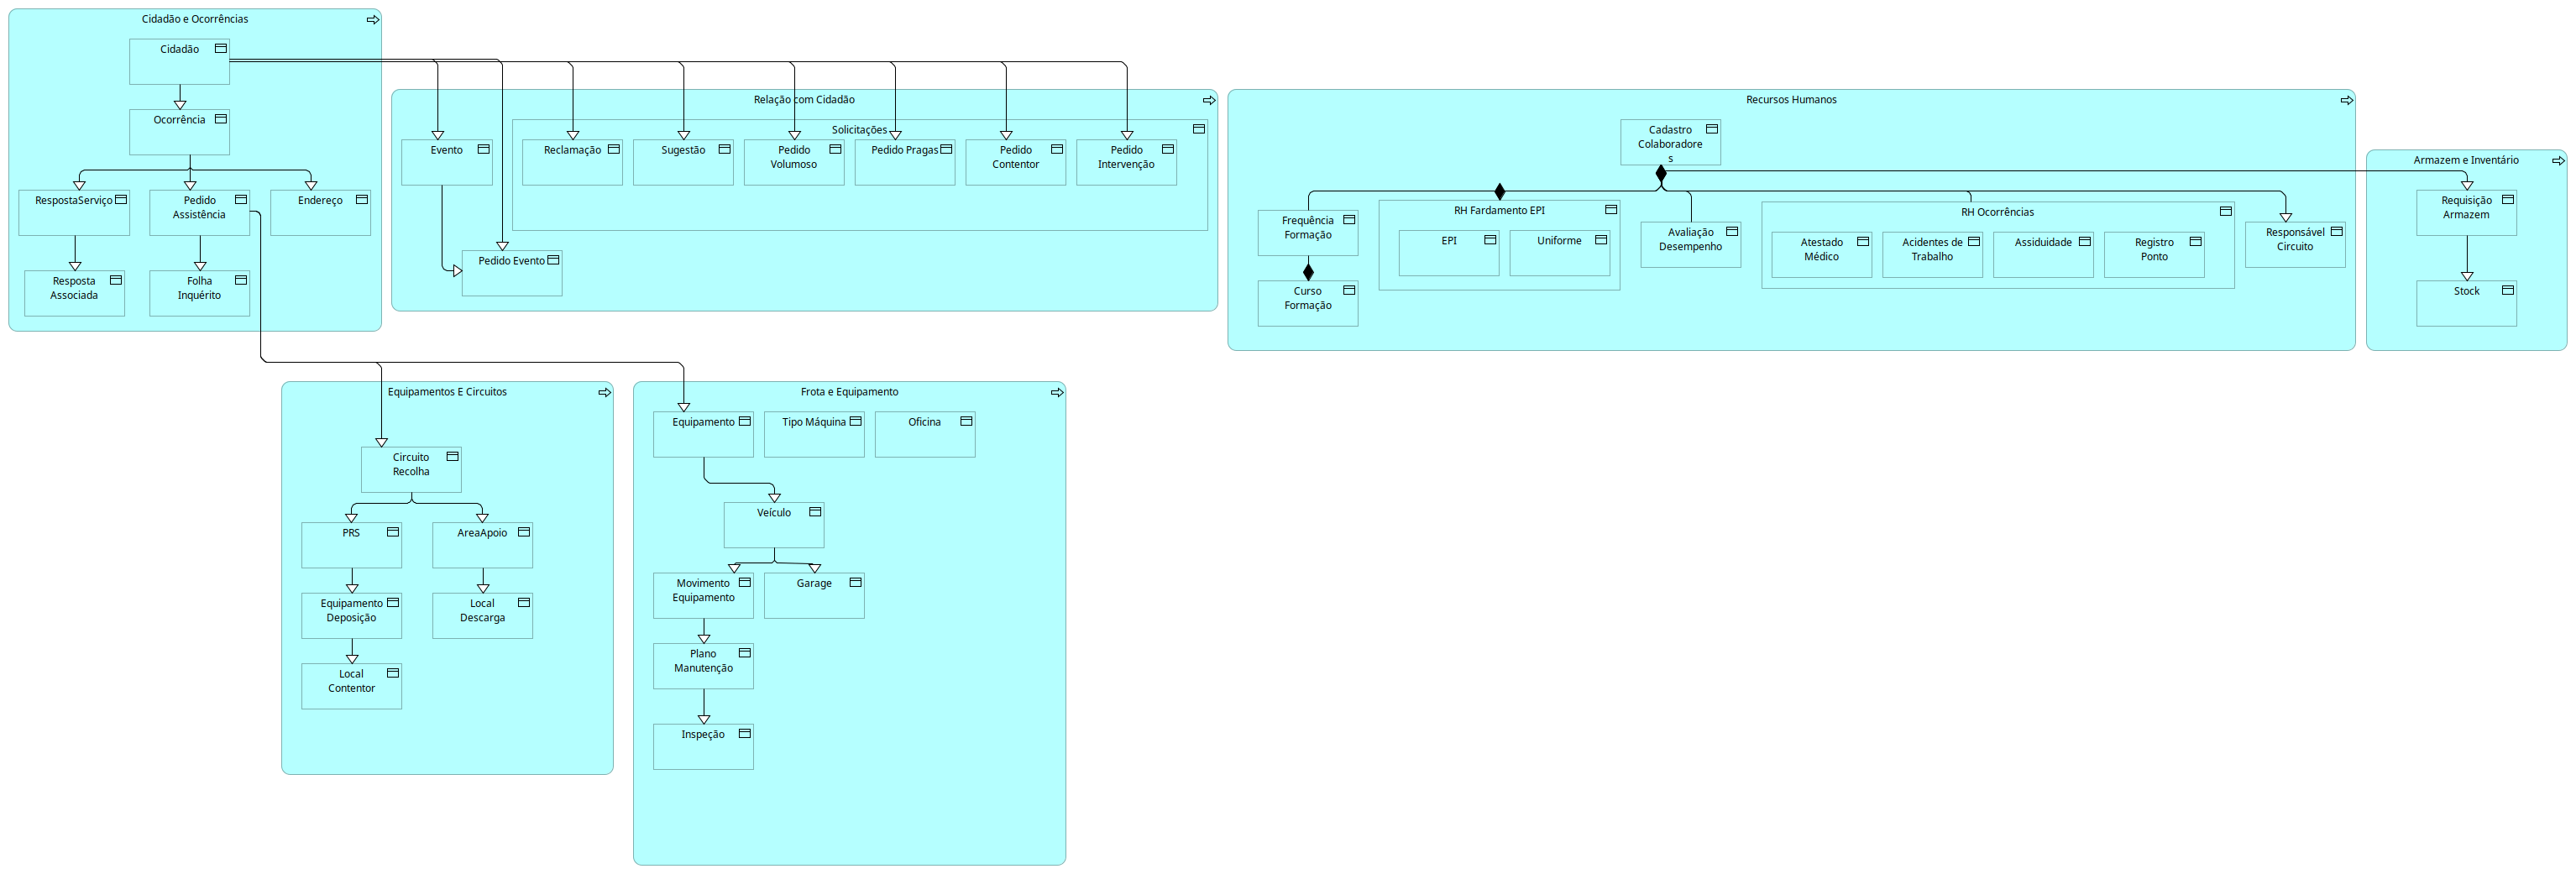
\includegraphics[width=\textwidth]{Q14.png}
        \caption{Domínios Informacionais e Entidades Relacionadas - Visão BSP}
        \label{fig:q14-domains}
    \end{figure}

    \textbf{Análise crítica:}
    \begin{itemize}
        \item \textbf{Silos funcionais:} O domínio de \textit{Armazém e Inventário} é maioritariamente isolado, com aplicações que apenas dialogam entre si, sem partilha eficaz com o domínio de Frota/Equipamentos. Isto dificulta a visibilidade global dos stocks de peças e o planeamento conjunto das operações de manutenção.
        \item \textbf{Sobreposições funcionais:} O domínio de \textit{Ocorrências e Cidadão} surge como exemplo de redundância – a mesma informação pode ser criada em múltiplos sistemas (ex: “Na Minha Rua Lx” vs backoffice de resíduos), levando a potenciais conflitos de atualização.
        \item \textbf{Dependências cruzadas:} Entidades como \textit{Viatura} e \textit{Equipamento} dependem simultaneamente de processos da Frota, da Manutenção e do Armazém, mas os fluxos não estão automatizados, havendo risco de desatualização.
        \item \textbf{Oportunidades de melhoria:} A integração da informação de formação, desempenho e ocorrências dos funcionários com o restante ciclo operacional (resíduos, frota, armazém) encontra-se subaproveitada, perdendo-se potencial analítico para gestão integrada.
    \end{itemize}

    Recomenda-se, para a evolução TO-BE, a centralização das entidades críticas e a adoção de mecanismos automáticos de integração de dados, mitigando os riscos identificados e potenciando o uso transversal da informação.

    \textbf{Conclusão:}
    A análise detalhada da matriz e do diagrama BSP evidencia a necessidade de quebrar silos, eliminar redundâncias e implementar processos de integração de dados. Isto permitirá à DMHU evoluir para uma arquitetura mais eficiente, com dados partilhados, maior automatização e melhor suporte à decisão.


    \section*{Questão 15 – Proposta de Arquitetura Aplicacional TO-BE (Estrutura)}
    \addcontentsline{toc}{section}{Q15 - Application Structure TO-BE}

    A arquitetura proposta para os próximos cinco anos reorganiza os sistemas aplicacionais em módulos interoperáveis, elimina silos identificados na matriz BSP e centraliza a gestão de entidades partilhadas. O diagrama seguinte demonstra a nova distribuição das aplicações, promovendo partilha, normalização e escalabilidade.

    \begin{figure}[H]
        \centering
        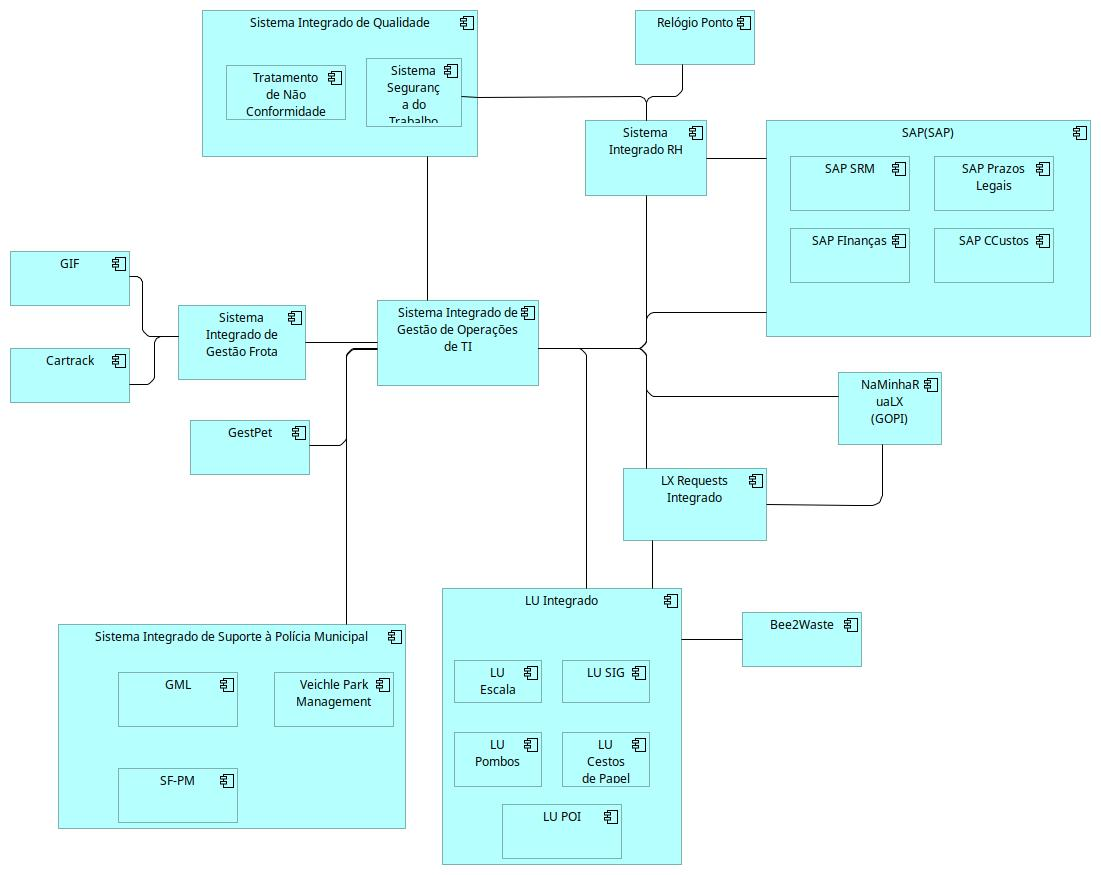
\includegraphics[width=0.98\textwidth]{Q15 - Application Structure.jpg}
        \caption{Estrutura proposta para a arquitetura aplicacional TO-BE}
        \label{fig:q15-app-structure-tobe}
    \end{figure}

    \textbf{Nota:} A proposta visa minimizar redundâncias, facilitar integrações futuras (ex: plataformas Smart City) e suportar evolução tecnológica sem fragmentação de dados.

    \section*{Questão 16 – Proposta de Arquitetura Aplicacional TO-BE (Utilização)}
    \addcontentsline{toc}{section}{Q16 - Application Usage TO-BE}

    A utilização das aplicações na arquitetura futura é apresentada de modo detalhado para cada área funcional (Administração, Cidadão, RH, Frota, Armazém, etc.), reflectindo a racionalização de módulos e fluxos.

    \begin{figure}[H]
        \centering
        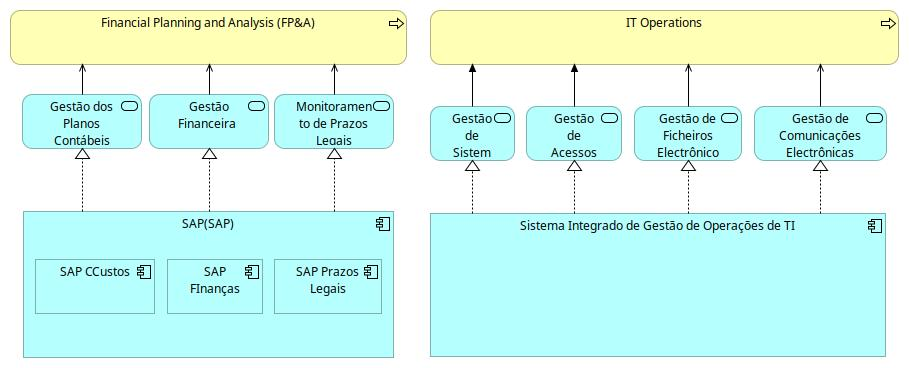
\includegraphics[width=0.48\textwidth]{Q16 - Application Usage - Admin Operations.jpg}
        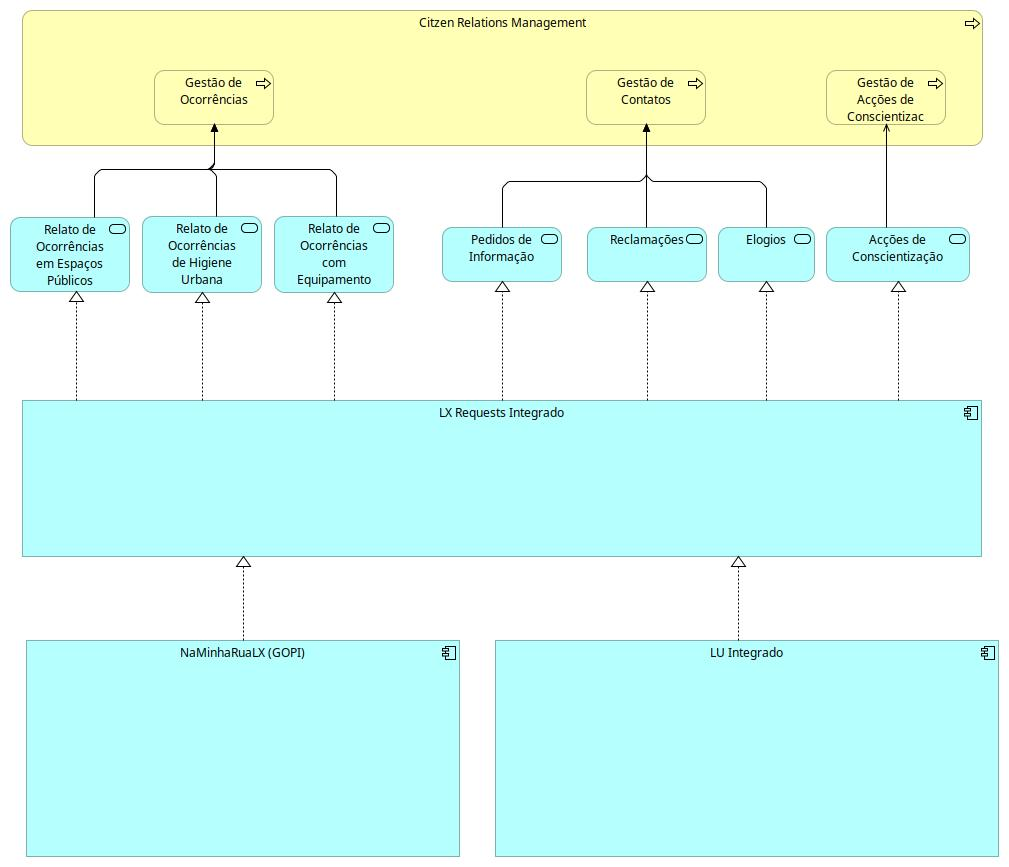
\includegraphics[width=0.48\textwidth]{Q16 - Application Usage - Citzen Relations Management.jpg}
        \caption{Utilização das aplicações TO-BE: Operações administrativas e Relações com o Cidadão}
        \label{fig:q16-usage-admin-cidadao}
    \end{figure}

    \begin{figure}[H]
        \centering
        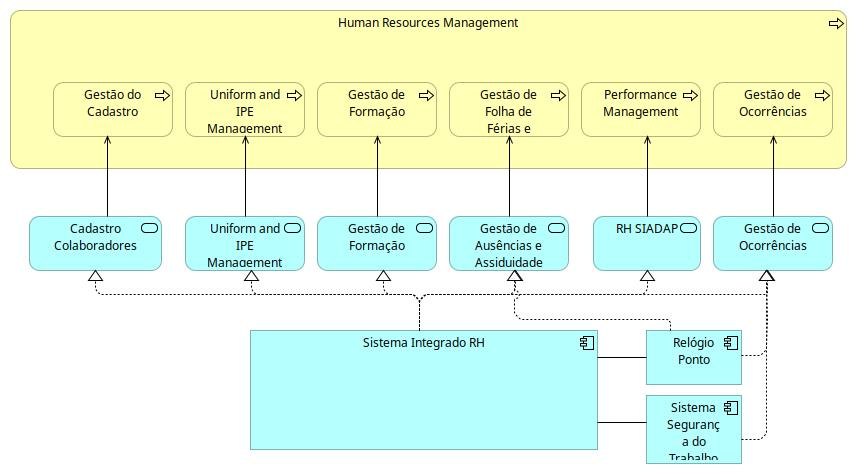
\includegraphics[width=0.48\textwidth]{Q16 - Application Usage - Human Ressources Management.jpg}
        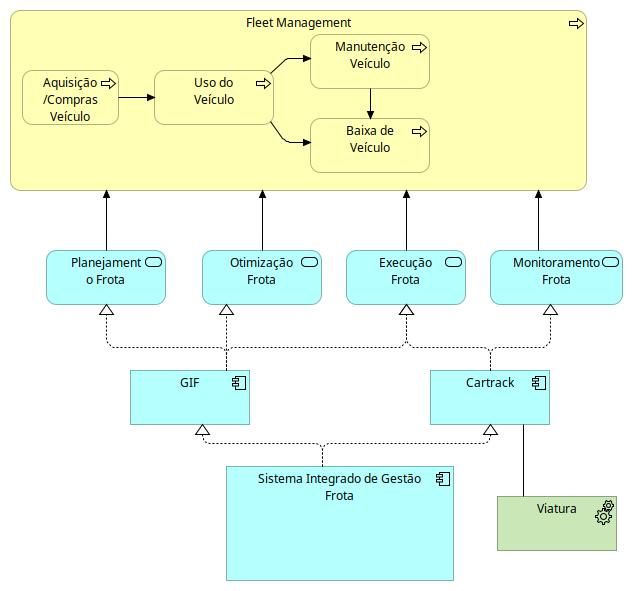
\includegraphics[width=0.48\textwidth]{Q16 - Application Usage - Fleet Management.jpg}
        \caption{Utilização das aplicações TO-BE: Recursos Humanos e Frota}
        \label{fig:q16-usage-rh-frota}
    \end{figure}

    \begin{figure}[H]
        \centering
        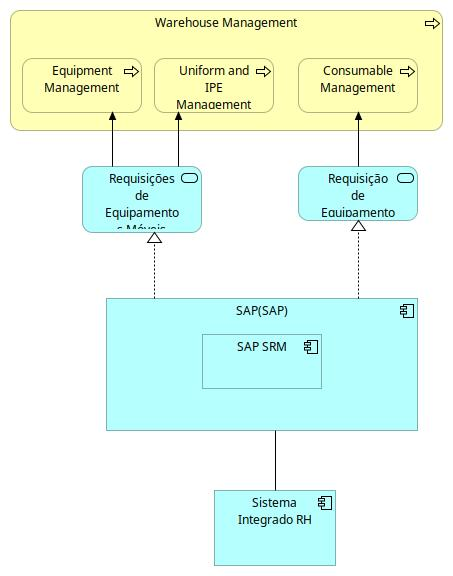
\includegraphics[width=0.48\textwidth]{Q16 - Application Usage - Warehouse Management.jpg}
        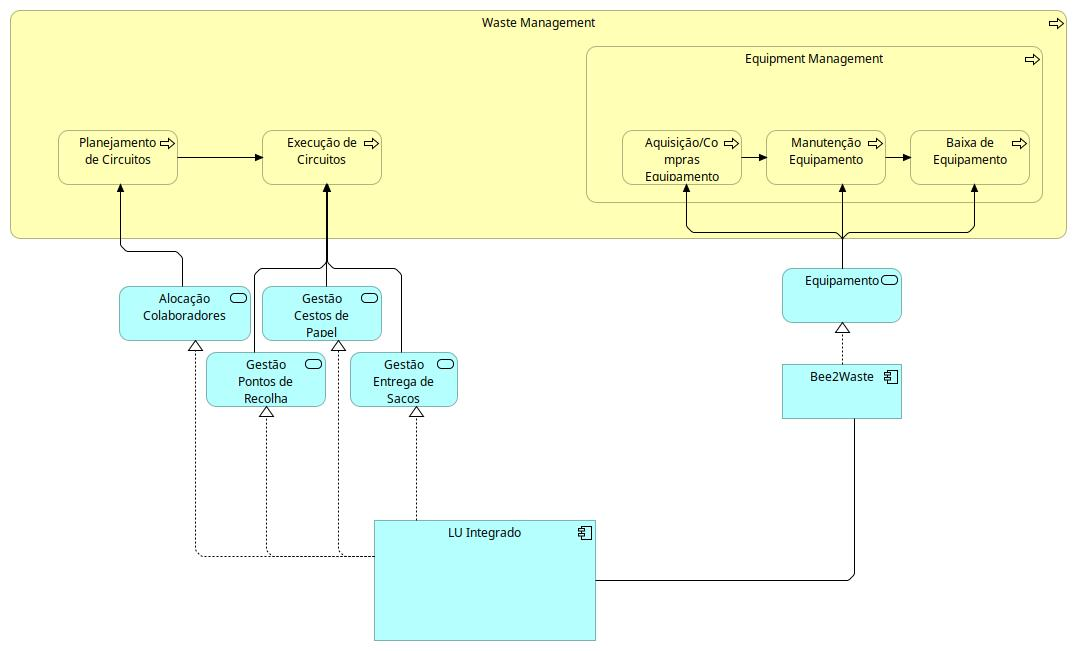
\includegraphics[width=0.48\textwidth]{Q16 - Application Usage - Waste Management.jpg}
        \caption{Utilização das aplicações TO-BE: Armazém e Gestão de Resíduos}
        \label{fig:q16-usage-armazem-residuos}
    \end{figure}

    \begin{figure}[H]
        \centering
        \includegraphics[width=0.48\textwidth]{Q16 - Application Usage - Miscelânea.jpg}
        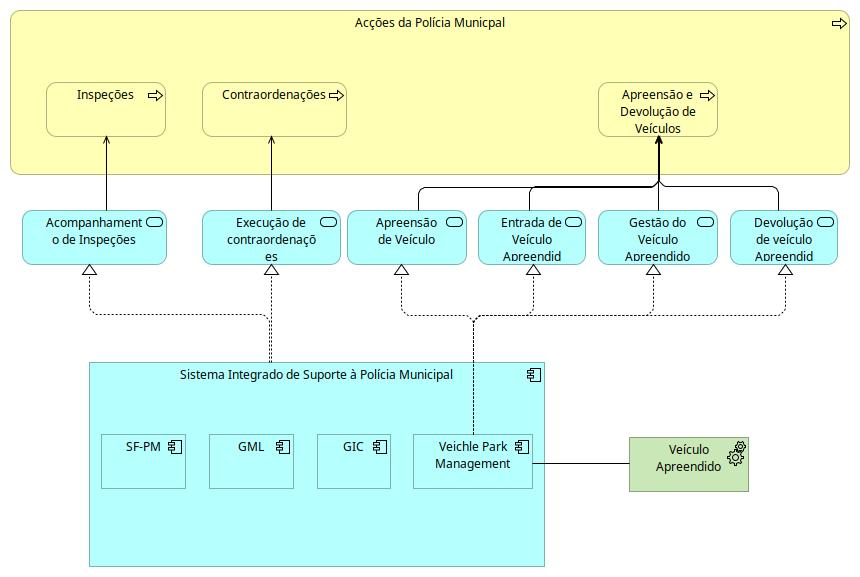
\includegraphics[width=0.48\textwidth]{Q16 - Application Usage - Municipal Police.jpg}
        \caption{Utilização das aplicações TO-BE: Miscelânea e Polícia Municipal}
        \label{fig:q16-usage-misc-pm}
    \end{figure}

    \textbf{Comentário:} A segregação de responsabilidades está agora claramente definida, facilitando monitorização, manutenção e integração multi-plataforma.

    \section*{Questão 17 – Proposta de Arquitetura Aplicacional TO-BE (Cooperação de Aplicações)}
    \addcontentsline{toc}{section}{Q17 - Application Cooperation TO-BE}

    A cooperação entre aplicações passa a ser realizada por interfaces normalizadas, integrando mecanismos de partilha de dados, workflows automáticos e serviços expostos a entidades externas.

    \begin{figure}[H]
        \centering
        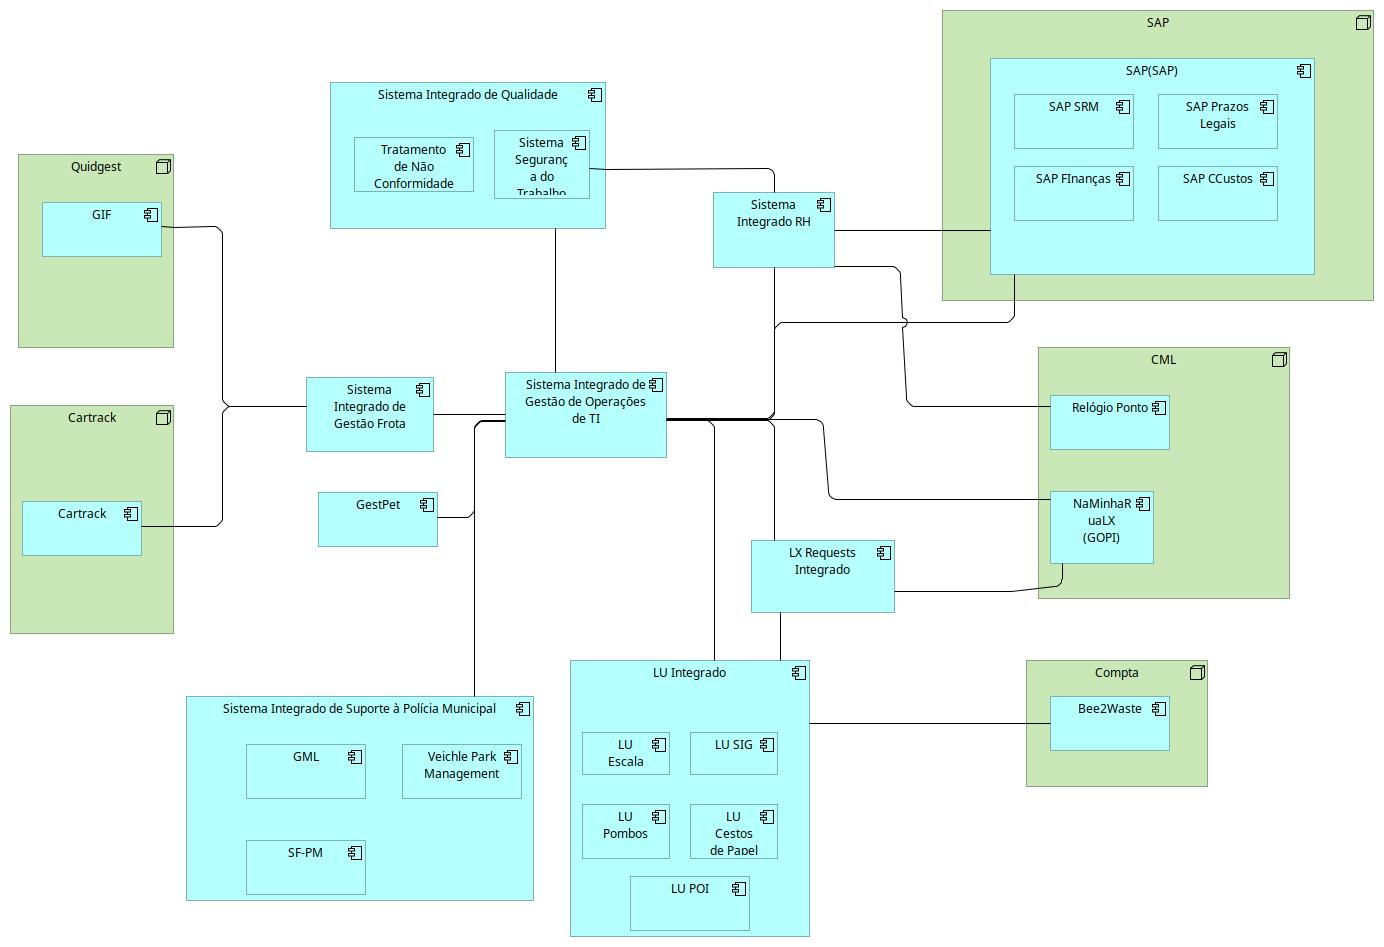
\includegraphics[width=0.95\textwidth]{Q17 - Application Cooperation.jpg}
        \caption{Cooperação entre aplicações na arquitetura TO-BE}
        \label{fig:q17-app-cooperation}
    \end{figure}

    \textbf{Nota:} Corrige-se assim o isolamento de silos e a falta de interoperabilidade diagnosticada na arquitetura AS-IS.

    \section*{Questão 18 – Proposta de Arquitetura Aplicacional TO-BE (Comportamento das Aplicações)}
    \addcontentsline{toc}{section}{Q18 - Application Behavior TO-BE}

    Nesta proposta, o comportamento das aplicações é modelado em detalhe para cada área funcional, clarificando fluxos, triggers e integrações, conforme se exemplifica nas figuras seguintes.

    \begin{figure}[H]
        \centering
        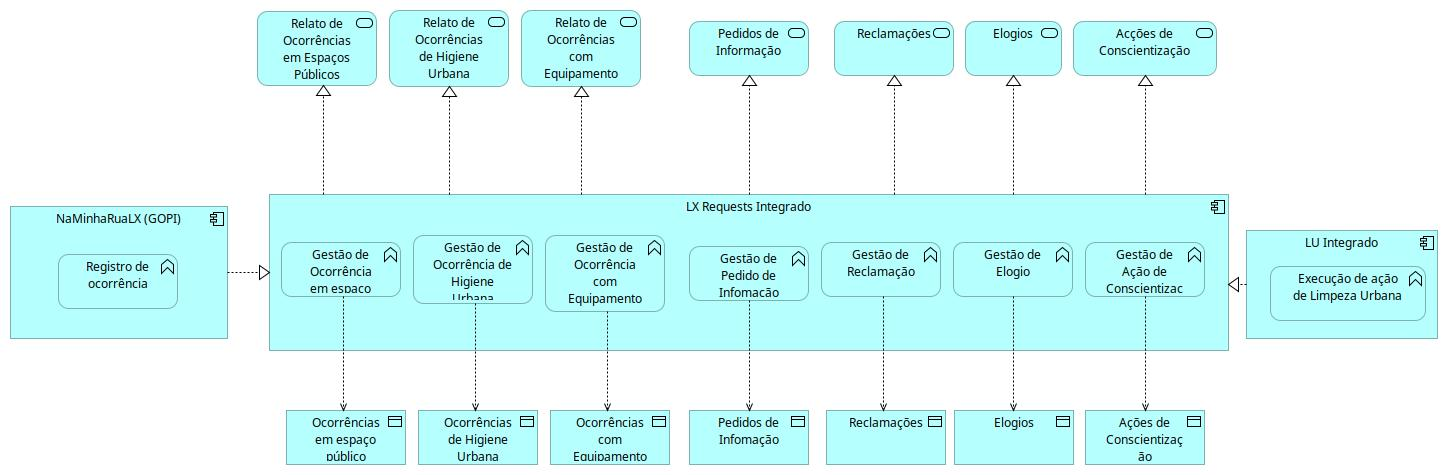
\includegraphics[width=0.48\textwidth]{Q18 - Application Behavior - Citzen Relations Management.jpg}
        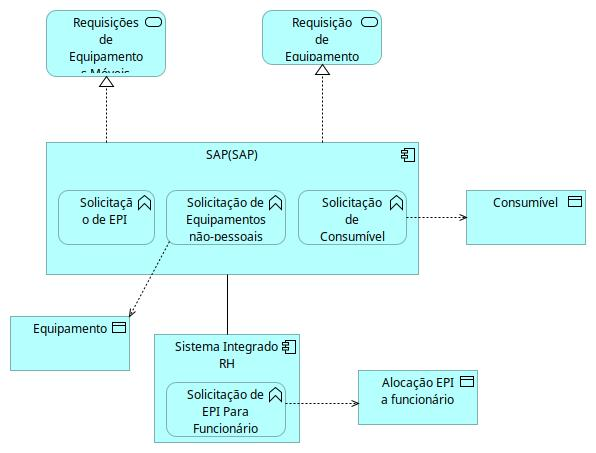
\includegraphics[width=0.48\textwidth]{Q18 - Application Behavior- Warehouse Management.jpg}
        \caption{Comportamento das aplicações: Relação com o Cidadão e Armazém}
        \label{fig:q18-behavior-cidadao-armazem}
    \end{figure}

    \begin{figure}[H]
        \centering
        \includegraphics[width=0.48\textwidth]{Q18 - Application Behavior- Admin Operations.jpg}
        \includegraphics[width=0.48\textwidth]{Q18 - Application Behavior- Fleet Management.jpg}
        \caption{Comportamento das aplicações: Operações Administrativas e Frota}
        \label{fig:q18-behavior-admin-frota}
    \end{figure}

    \begin{figure}[H]
        \centering
        \includegraphics[width=0.48\textwidth]{Q18 - Application Behavior- Human Ressources Management.jpg}
        \includegraphics[width=0.48\textwidth]{Q18 - Application Behavior - Miscelânea.jpg}
        \caption{Comportamento das aplicações: Recursos Humanos e Miscelânea}
        \label{fig:q18-behavior-rh-misc}
    \end{figure}

    \begin{figure}[H]
        \centering
        \includegraphics[width=0.48\textwidth]{Q18 - Application Behavior - Waste Management.jpg}
        \includegraphics[width=0.48\textwidth]{Q18 - Application Behavior- Municipal Police.jpg}
        \caption{Comportamento das aplicações: Gestão de Resíduos e Polícia Municipal}
        \label{fig:q18-behavior-residuos-pm}
    \end{figure}

    \textbf{Nota:} Foram corrigidas ambiguidades na definição de triggers, passando a estar claramente descritas as interações internas e externas, e garantindo rastreabilidade dos fluxos automatizados.

    \section*{Questão 19 – Proposta de Infraestrutura de Processamento TO-BE}
    \addcontentsline{toc}{section}{Q19 - Processing Infrastructure TO-BE}

    A infraestrutura de processamento futura adota uma abordagem híbrida (on-premises/cloud), prevendo crescimento e flexibilidade. Estão previstos mecanismos de alta disponibilidade, balanceamento e tolerância a falhas.

    \begin{figure}[H]
        \centering
        \includegraphics[width=0.95\textwidth]{Q19 - Processing Infraestructure Proposal.jpg}
        \caption{Infraestrutura de processamento proposta (TO-BE)}
        \label{fig:q19-processing-tobe}
    \end{figure}

    \textbf{Comentário:} Esta arquitetura elimina single points of failure identificados no modelo AS-IS e facilita futuras integrações com sistemas externos.

    \section*{Questão 20 – Proposta de Infraestrutura de Armazenamento TO-BE}
    \addcontentsline{toc}{section}{Q20 - Storage Infrastructure TO-BE}

    A nova arquitetura de storage contempla redundância de dados, segmentação lógica por domínio e suporte nativo para integrações de business intelligence.

    \begin{figure}[H]
        \centering
        \includegraphics[width=0.95\textwidth]{Q20 - Storage Infraestructure Proposal.jpg}
        \caption{Infraestrutura de armazenamento proposta (TO-BE)}
        \label{fig:q20-storage-tobe}
    \end{figure}

    \textbf{Nota:} Os dados críticos passam a ser replicados, classificados e acessíveis de forma controlada, corrigindo deficiências de partilha e segurança do modelo anterior.

    \section*{Questão 21 – Proposta de Infraestrutura de Comunicação TO-BE}
    \addcontentsline{toc}{section}{Q21 - Communication Infrastructure TO-BE}

    A infraestrutura de comunicação é redesenhada para garantir integração com sistemas internos e externos, segurança na troca de dados e conformidade com normas europeias.

    \begin{figure}[H]
        \centering
        \includegraphics[width=0.48\textwidth]{Q21 - Communication Infrastructure Proposal - 3rd Party Systems.jpg}
        \includegraphics[width=0.48\textwidth]{Q21 - Communication Infrastructure Proposal - CML Systems.jpg}
        \caption{Infraestrutura de comunicação proposta – Sistemas internos e externos}
        \label{fig:q21-comms-tobe}
    \end{figure}

    \textbf{Nota:} Este modelo previne pontos de falha e garante escalabilidade nas integrações.

    \section*{Questão 22 – Relação entre Infraestrutura e Aplicações TO-BE}
    \addcontentsline{toc}{section}{Q22 - Infrastructure and Application Usage TO-BE}

    Mapeia-se nesta fase a ligação entre cada aplicação e os componentes de infraestrutura onde é executada, reforçando visibilidade e rastreabilidade operacionais.

    \begin{figure}[H]
        \centering
        \includegraphics[width=0.48\textwidth]{Q22 - Relation Between Infraestructure and Applications - 3rd Party Systems.jpg}
        \includegraphics[width=0.48\textwidth]{Q22 - Relation Between Infraestructure and Applications - CML Systems.jpg}
        \caption{Relação infraestruturas-aplicações: sistemas internos e de terceiros}
        \label{fig:q22-infra-app}
    \end{figure}

    \textbf{Nota:} Foram eliminadas ambiguidades e corrigidos mapas de dependências cruzadas.

    \section*{Questão 23 – Deployment das Aplicações na Infraestrutura}
    \addcontentsline{toc}{section}{Q23 - Application Deployment}

    O modelo seguinte representa o deployment físico e lógico das aplicações nas infraestruturas, incluindo agrupamentos por domínio funcional e zonas de segurança.

    \begin{figure}[H]
        \centering
        \includegraphics[width=0.95\textwidth]{Q23 - Implementation and Deployment.jpg}
        \caption{Deployment das aplicações na infraestrutura proposta}
        \label{fig:q23-deployment}
    \end{figure}

    \textbf{Comentário:} Esta abordagem facilita migração, manutenção e recuperação de desastres.

    \section*{Questão 24 – Limitações e Decisões do Projeto}
    \addcontentsline{toc}{section}{Q24 - Project Limitations and Decisions}

    \textbf{Limitações:}
    \begin{itemize}
        \item Restrição orçamental para aquisição de licenciamento e infraestruturas cloud/híbridas.
        \item Necessidade de gestão da mudança junto dos recursos humanos, devido à alteração de processos e adoção de novas ferramentas.
        \item Dependência de integrações com sistemas legados e terceiros, sujeitos a disponibilidade e normas externas.
        \item Risco de resistência organizacional, especialmente em áreas menos digitalizadas.
    \end{itemize}

    \textbf{Decisões críticas:}
    \begin{itemize}
        \item Centralização de dados críticos em plataformas interoperáveis, reduzindo silos.
        \item Adoção de standards de interoperabilidade (ex.: BPMN 2.0, ArchiMate 3, UML 2.0).
        \item Implementação faseada, priorizando processos core e áreas com maior impacto na qualidade do serviço.
        \item Previsão de evolução futura: flexibilidade para adoção de tecnologias emergentes (cloud, IoT, Smart City).
    \end{itemize}

    \textbf{Nota Final:} A abordagem adotada para este projeto visou responder aos problemas identificados no diagnóstico AS-IS, corrigir fragilidades na arquitetura e preparar a DMHU para os desafios futuros de modernização e integração numa verdadeira Smart City.

    \section*{Conclusão}
    \addcontentsline{toc}{section}{Conclusão}

    O presente trabalho permitiu realizar um diagnóstico aprofundado à arquitetura de sistemas de informação da DMHU, destacando pontos fortes, fragilidades e oportunidades de evolução. A análise detalhada das entidades, processos, aplicações e infraestruturas, complementada por uma abordagem crítica às matrizes CRUD e à segmentação de domínios, permitiu evidenciar silos, redundâncias e lacunas funcionais relevantes para a eficiência operacional.

    A proposta de arquitetura TO-BE apresentada neste relatório responde aos principais desafios identificados: racionaliza e integra os sistemas, centraliza a governação de dados, elimina sobreposições funcionais e cria bases para futuras iniciativas de digitalização, automação e inteligência organizacional. Destaca-se a importância da adoção de standards, da implementação faseada e da gestão da mudança organizacional para o sucesso da transformação.

    Como oportunidades futuras, salienta-se a integração plena com plataformas de Smart City, a utilização de soluções de análise avançada de dados (analytics, BI), e a contínua monitorização e adaptação da arquitetura, assegurando a sua sustentabilidade e adequação à missão de serviço público da DMHU.



    \newpage
    \nocite{*}
    \printbibliography
\end{document}